\chapter{Marco Teórico}\label{cap:05EstudioPrevio}

Este capítulo presenta el marco teórico sobre OHDSI:  \ref{sec:05intro} Introducción breve al capítulo,  \ref{sec:05OHDSI} Qué es OHDSI,  \ref{sec:05Evidencia} Cómo generar evidencia, \ref{sec:05herramientas} Qué herramientas ofrece y \ref{sec:05conclusion} Breve conclusión final.

\section{Introducción} \label{sec:05intro}
%El objetivo es dar a concoer todos los conceptos teóricos de OHDSI y ATLAS. Quién quiera utilizar ATLAS debe conocer OHDSI, debe conocer el CDM, el Vocab, otras herramientas... Son conceptos fundamentales.

La organización Observational Health Data Science and Informatics (OHDSI) es muy importante para el TFG por ser la proveedora de la herramienta de análisis ATLAS, núcleo central del trabajo, y por la relevancia que ha adquirido a nivel europeo en los últimos años.

Por tanto, en este capítulo se pretende dar a conocer al lector el ecosistema completo de la organización que provee la herramienta, en cuanto a los aspectos más generales como los más específicos. No se puede entender ATLAS sin entender OHDSI porque las herramientas no están aisladas sino que forman parte de un ecosistema dependiente entre sí. Todas estas dependencias y conceptos necesarios se exponen en este capítulo para generar un conocimiento profundo subyacente al caso práctico (véase \ref{cap:08pruebas}) y para poder volver a estos conceptos básicos cuando fuere necesario.

\section{¿Qué es OHDSI?} \label{sec:05OHDSI}

OHDSI, pronunciado en inglés ''Odyseey'', son las siglas de \textit{Observational Health Data Science and Informatics}. OHDSI es una organización colaborativa de ciencia abierta cuyo propósito, de forma muy resumida, es mejorar la investigación cientifico-sanitaria a través de la ciencia de datos y la informática clínica. No obstante, no es solo una organización, sino una comunidad global abierta a todo el que esté interesado y alineado con su misión, visión y objetivos. 

La comunidad se asigna por tanto la misión de ''mejorar la salud empoderando a una comunidad para generar de manera colaborativa evidencia que promueva mejores decisiones de salud y una mejor atención'', y comparte la visión de ''un mundo en el que la investigación observacional produzca una comprensión integral de la salud y la enfermedad'' \cite{OHDSIwebsite}\cite{OHDSIbook}. 

Por otra parte, en El Libro de OHDSI la organización se define así misma como ''una comunidad de ciencia abierta que tiene como objetivo mejorar la salud empoderando a la comunidad para generar de manera colaborativa evidencia que promueva mejores decisiones de salud y mejor atención'' \cite{OHDSIbook}. %La web oficial presenta otra definición algo diferente, se presenta como ''una colaboración de ciencia abierta, interdisciplinaria y de múltiples partes interesadas para resaltar el valor de los datos de salud a través de análisis a gran escala'' \cite{OHDSIwebsite}.

\begin{figure}[H]
    \centering
    
\includegraphics[width=0.90\textwidth]{figures/OHDSIbanner.png}
    \caption{Banner de OHDSI. Extraído de web oficial \cite{OHDSIwebsite}}
    \label{fig:OHDSIbanner}
\end{figure}

Por tanto, a la pregunta sobre \textit{qué es OHDSI} se puede responder apoyándose en cuatro características fundamentales: (i)  una comunidad o red colaborativa, (ii) de ciencia abierta, (iii) estandarizada y (iv) con la finalidad de promover la extracción de evidencia a partir de datos clínicos.

\begin{enumerate}[label=\roman*.]
    \item \textbf{Una comunidad o red colaborativa}. La organización es una comunidad, es decir, se presenta abierta a la incorporación de todo aquel que esté comprometido con su misión. Además se muestra siempre abierta e interesada en la incorporación de nuevos colaboradores, lo que muestran constantemente con el eslogan \textit{''Join the Journey''}, en español, ''únete a la aventura'' (véase Figura \ref{fig:joinTheJourney}). Además la organización distribuye a sus colaboradores en nodos por países y en grupos de trabajo según los diferentes componentes de OHDSI. 
    
\begin{figure}[H]
    \centering
    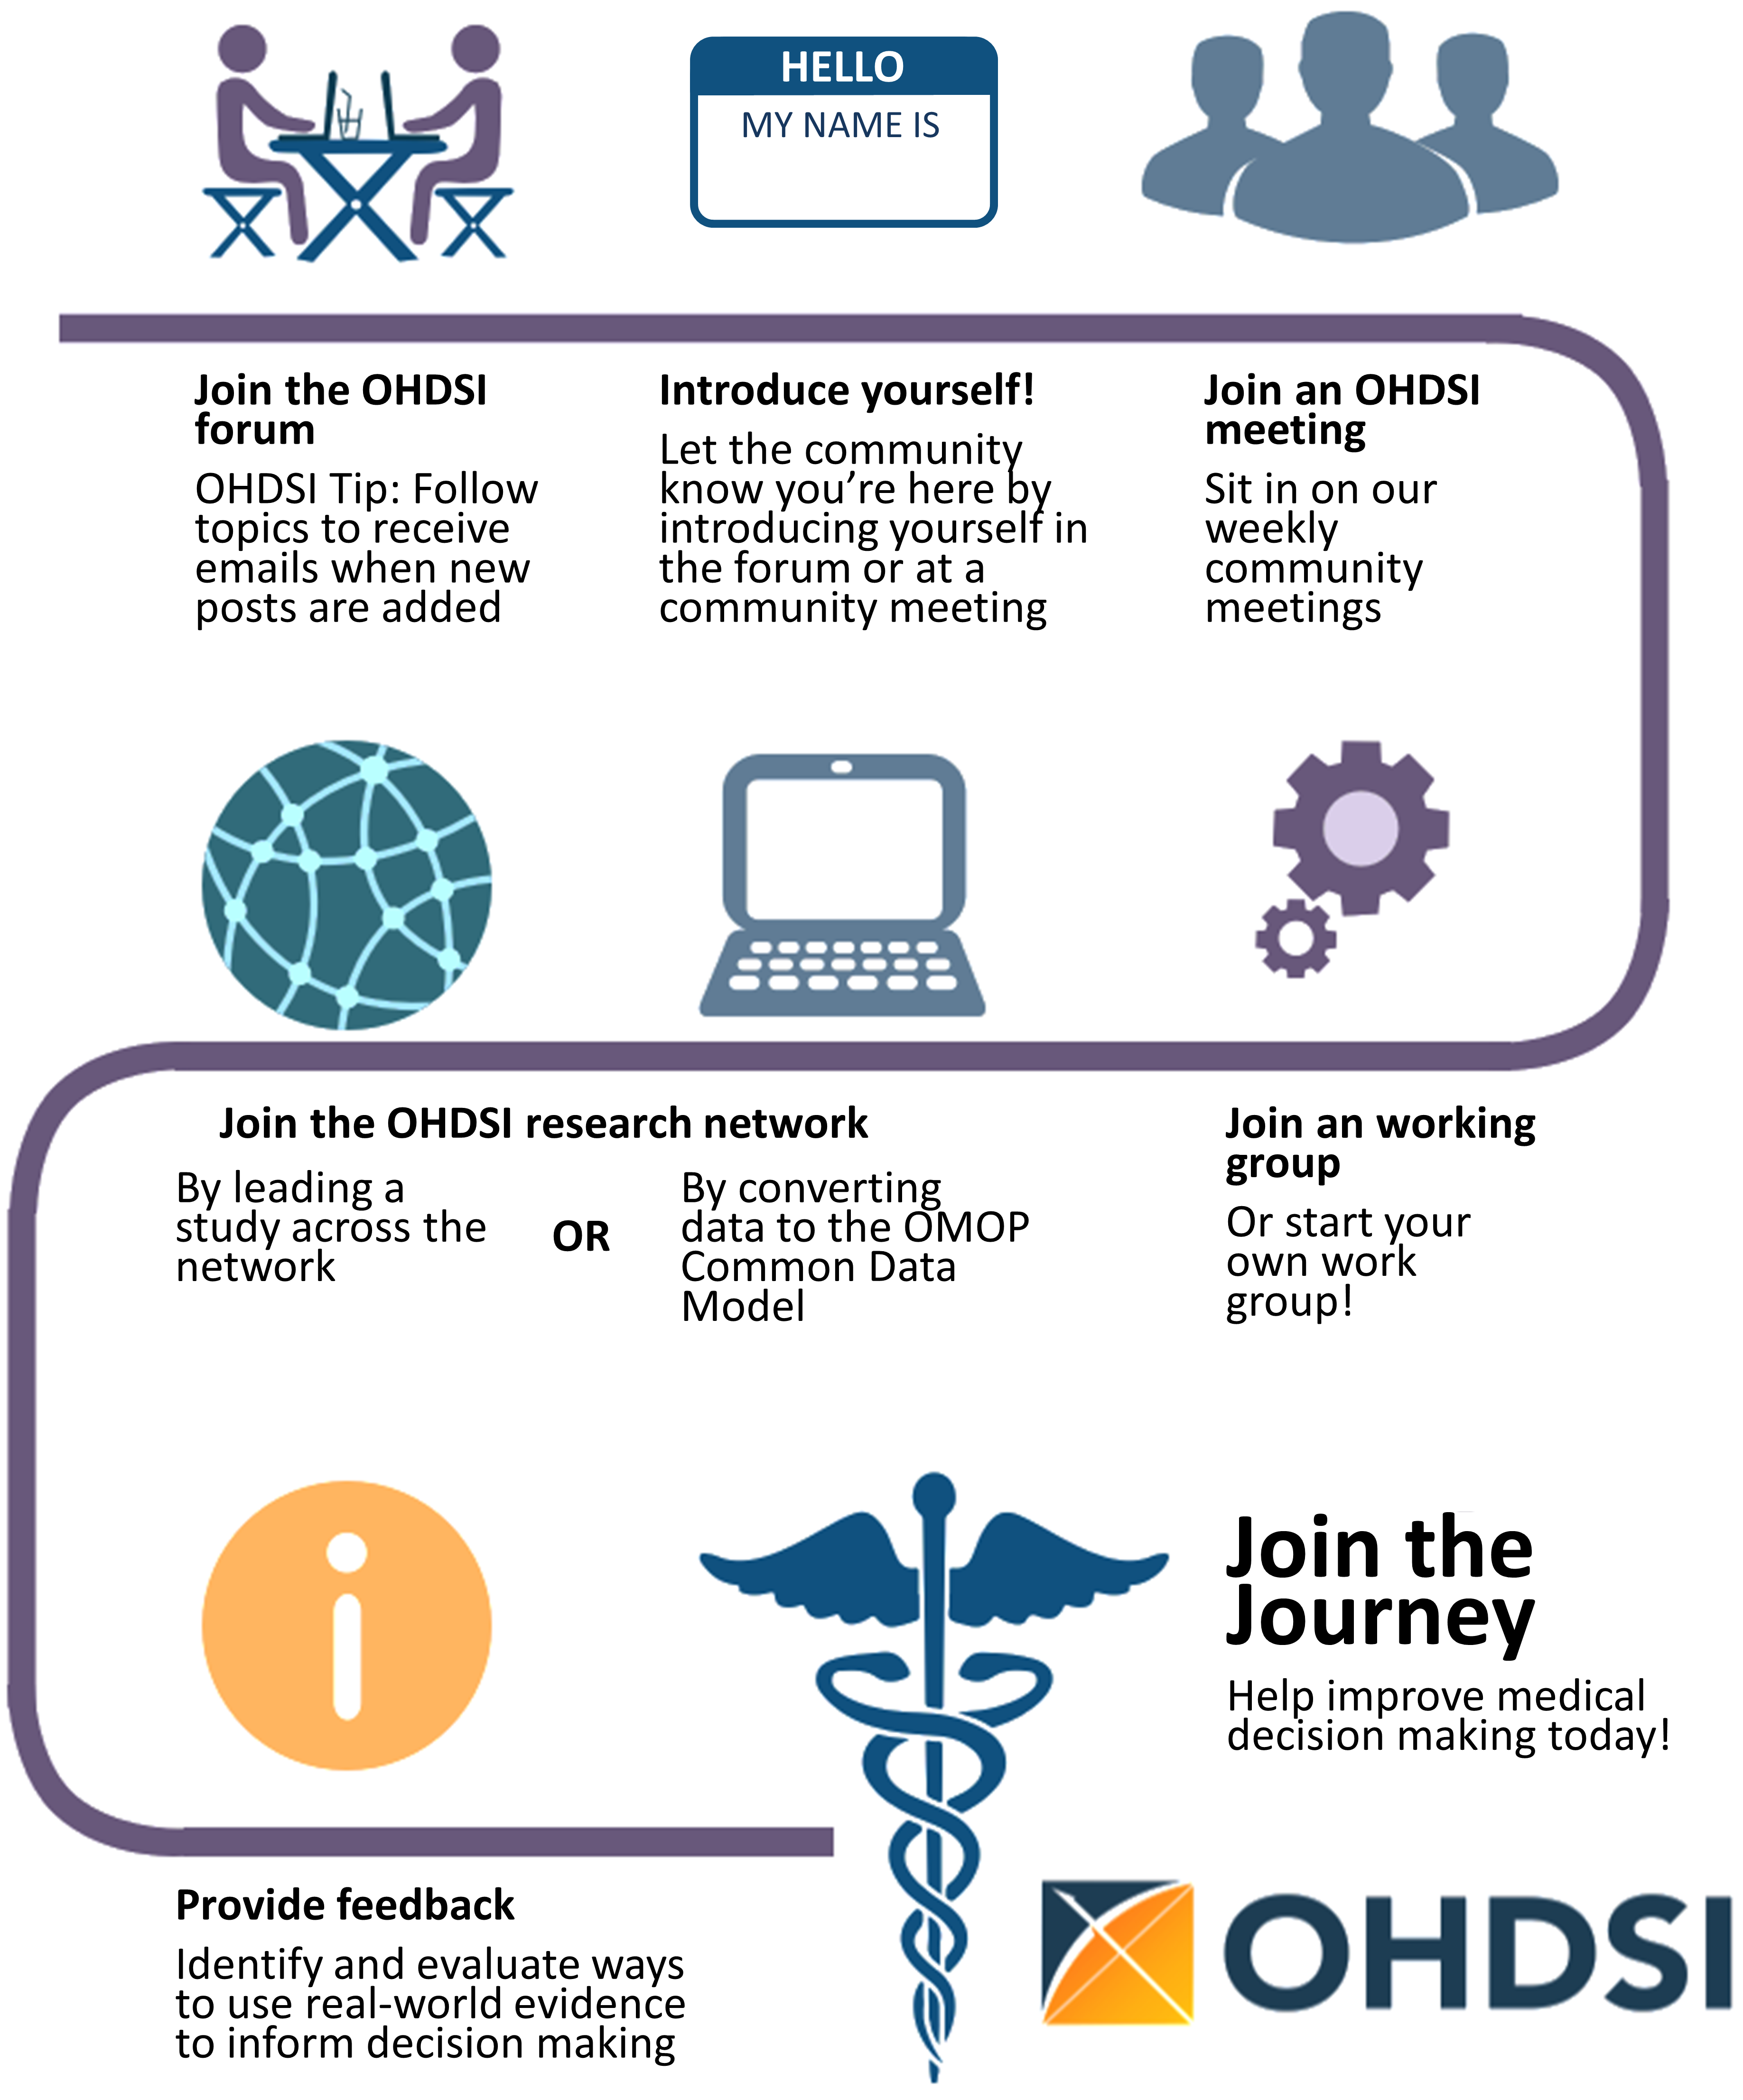
\includegraphics[width=0.50\textwidth]{figures/joinTheJourney.png}
     \caption{\textit{Join the Journey}. Extraído del Libro de OHDSI \cite{OHDSIbook}}
    \label{fig:joinTheJourney}
\end{figure}
    
    %Esta red de colaboradores busca componerse de un gran equipo multidisciplinar, pues se entiende que el propósito que persigue la organización es tan extenso y complejo que es complicado que una única persona albergue todo el conocimiento técnico para desarrollar a la perfección cada etapa de un proyecto, por ello hace especial hincapié en recibir colaboradores expertos en diferentes materias pero que contribuyan al proyecto común de OHDSI.

    \item \textbf{Ciencia abierta}. La forma de trabajar de la organización es muy importante, puesto que promueve la colaboración entre las organziaciones y la participación a través de la ciencia abierta.

    Todos los eventos, publicaciones, herramientas y documentación que elabora OHDSI están disponibles públicamente y de forma gratuita en internet, para que pueda unirse quien quiera (en el caso de los eventos) o consultarse y usarse en cualquier momento (en caso de las herramientas e información). Las dos vías de información por excelencia sobre OHDSI son su página web \cite{OHDSIwebsite} y el \textit{Libro de OHDSI} \cite{OHDSIbook}. Otras vías de información son a través de publicaciones científicas \cite{OHDSIpublications}, tutoriales para principiantes, grabaciones de las reuniones semanales de la comunidad o las conferencias anuales a través de su canal de youtube \cite{OHDSIyt}, canales de mensajería abierta como discord \cite{OHDSIdiscordInvitation} o MS Teams \cite{OHDSIofficeForm}, cientos de repositorios de github con información técnica de cada herramienta \cite{OHDSIgithub} y los foros de la comunidad para solventar dudas y preguntas \cite{OHDSIforums}, entre otros.

    Además, OHDSI asegura la fiabilidad, accesibilidad, interoperabilidad y reproducibilidad de sus estudios a través del cumplimiento de los principios FAIR, que desarrolla en gran extensión en la sección 3.7 de su libro \cite{OHDSIbook}.

    \item \textbf{Estandarización}. OHDSI aboga por estandarizar los modelos de datos y la metodología de la investigación médica a un modelo común, con la finalidad de aumentar la interoperabilidad entre los sistemas y organizaciones sanitarias a nivel mundial.
    
    Esta idea se presenta en el Symposium de 2023 con un ejemplo muy intuitivo: la conexión a la corriente eléctrica a través de una plancha. La conexión de la plancha sería la realización de un estudio sobre unos datos, que serían el enchufe a la corriente eléctrica, siendo el objetivo establecer un enchufe estándar que permita la conexión de la plancha a la corriente eléctrica en cualquier lugar del mundo, es decir, la realización de un estudio siguiendo una misma estructura en cualquier lugar del mundo.

\begin{figure}[H]
    \centering
    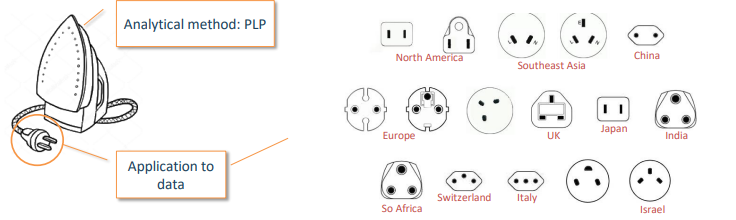
\includegraphics[width=0.60\textwidth]{figures/plancha1.png}
     %\caption{Ejemplo de la plancha con diferentes enchufes. Extraído de la web oficial \cite{OHDSIwebsite}}
    \label{fig:plancha1}
\end{figure}
\begin{figure}[H]
    \centering
    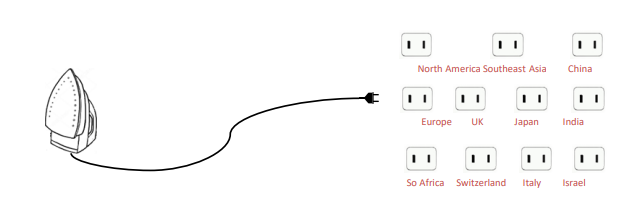
\includegraphics[width=0.70\textwidth]{figures/plancha2.png}
     \caption{Ejemplo de la plancha. Extraído de la web oficial \cite{OHDSIwebsite}}
    \label{fig:plancha2}
\end{figure}

    \item \textbf{Extracción de evidencia a partir de datos clínicos}. Es importante destacar la finalidad de OHDSI de, no solo recopilar y almacenar la información clínica, sino también extraer información o evidencia de ella. 
    %La organización identifica la dificultad de extraer información trascendental de los datos clíncos debido a sus distintas morfologías y estructuras en las que son recogidos. 
    Este es el propósito final y enfrenta muchos desafíos debido a la disparidad de los datos y técnicas de análisis. 
    
    El proceso de extracción de evidencia no es sencillo, como se muestra en la Figura \ref{fig:drawinJourney}, y parte en un extremo de las diferentes bases de datos del mundo real (RWD) (véase \ref{sec:01Contexto}) hacia la obtención fiable de evidencia del mundo real (RWE). Este recorrido debe atravesar un proceso de ETL para estandarizar las bases de datos al modelo común de OMOP, la integración con el vocabulario y el análisis técnico en sí que permita extraer la evidencia. Por suerte, la organización también proporciona un conjunto de herramientas (véase \ref{sec:05herramientas}) para realizar más sencillamente todo el recorrido.

\begin{figure}[H]
    \centering
    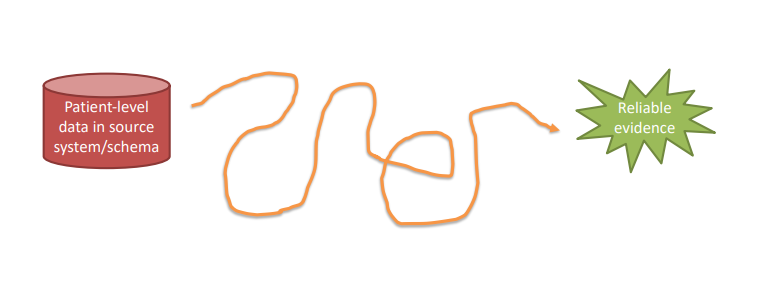
\includegraphics[width=0.80\textwidth]{figures/drawinJourney.png}
     \caption{Dibujo del proceso de extracción de evidencia. Extraído de la web oficial \cite{OHDSIwebsite}}
    \label{fig:drawinJourney}
\end{figure}



\end{enumerate}

\subsection{Historia}

Es común encontrar en internet los términos OHDSI y OMOP (\textit{Observational Medical Outcomes Partnership}), utilizados de forma casi indistintiva. Si bien es verdad que OMOP se suele asociar mayoritariamente al CDM (\textit{Common Data Model}) también OHDSI mantiene gran relación con este modelo común de datos. Entonces, ¿cuál es la relación entre estas dos entidades? Pues bien, la iniciativa de OHDSI se originó en 2014, posterior al proyecto OMOP, que finalizó en 2013, pues la relación que guardan estas dos entidades es filial, OHDSI es la sucesora de OMOP. 

OMOP nació en 2008 como una asociación público-privada presidida por la Administración de Alimentos y Medicamentos de EE. UU. con el objetivo de establecer buenas prácticas en estudios observacionales retrospectivos. El proyecto además fue administrado por la Fundación de los Institutos Nacionales de Salud y financiado por un consorcio de compañías farmacéuticas en colaboración con otros investigadores académicos y socios de datos de salud \cite{stang2010advancing}. El propósito inicial de OMOP era impulsar la ciencia de la vigilancia activa de la seguridad de los productos médicos mediante el análisis de datos observacionales de atención médica \cite{stang2010advancing}. Sin embargo, durante su desarrollo, se enfrentó a los desafíos técnicos de llevar a cabo investigaciones en bases de datos observacionales muy heterogéneas entre sí.

El resultado fue el desarrollo de un Modelo Común de Datos (CDM) como un mecanismo para estandarizar la estructura, el contenido y la semántica de los datos observacionales y hacer posible escribir código de análisis estadístico que fuera reutilizable para estudios en distintas fuentes de datos \cite{overhage2012validation}. Los experimentos de OMOP demostraron la viabilidad de establecer un CDM que además reuniese diferentes vocabularios estandarizados, reuniendo en un mismo estándar diversos tipos de datos de diferentes entornos de atención y representados por diferentes vocabularios de origen. Esta característica facilitó la colaboración y aumentó el interés entre diferentes instituciones lo que promovió o un enfoque de ciencia abierta \cite{OHDSIbook}. OMOP puso todo su trabajo a disposición del público, incluidos diseños de estudio, estándares de datos, código de análisis y hallazgos empíricos, para mejorar la transparencia y fomentar la confianza en su investigación. 

Al término del proyecto, el Modelo Común de Datos (CDM) de OMOP había evolucionado hasta respaldar un abanico  amplísimo de aplicaciones analíticas, incluida la efectividad comparativa de intervenciones médicas y políticas de todo el sistema de salud, no solo de la industria farmacéutica, por tanto, el equipo de investigación acordó que el fin de dicho proyecto debería ser el origen de uno nuevo. a partir de esta idea nació OHDSI \cite{OHDSIbook}.

\subsection{Actualidad}

Por tanto, lo que nació en 2014 como la continuación del proyecto OMOP ha evolucionado hasta convertirse en una extensa red colaborativa global.  En la actualidad, la comunidad de OHDSI cuenta con la participación de más de tres mil colaboradores distribuidos en 80 países.

\begin{figure}[H]
    \centering
    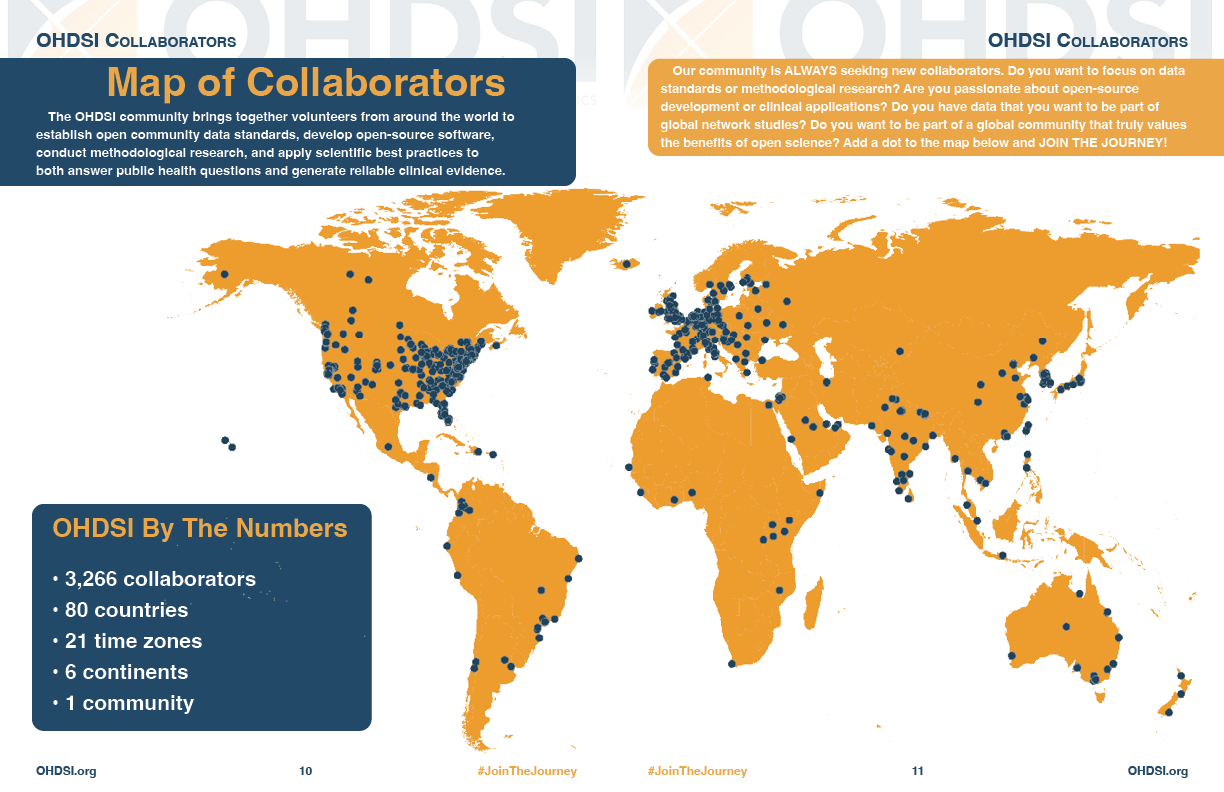
\includegraphics[width=0.80\textwidth]{figures/OHDSIcollaborators.png}
     \caption{Mapa de colaboradores de OHDSI. Extraído de la web oficial \cite{OHDSIwebsite}}
    \label{fig:OHDSIcollaborators}
\end{figure}

Además, tal y como se presenta en \ref{sec:01EstadoArte}, desde que se inició su colaboración con EHDEN (European Health Data Evidence) en 2020, OHDSI está adquiriendo cada vez mayor relevancia a nivel europeo. Ejemplo de ello es la celebración, este mes de junio, en Rotterdam del quinto Symposium Europeo de OHDSI (véase Figura \ref{fig:bannerSymposyum2024}), que tiene el fin de reunir a los expertos y miembros de la comunidad para presentar los grandes proyectos nacionales y europeos que se están realizando en toda europa con las herramientas de la comunidad.

\begin{figure}[H]
    \centering
    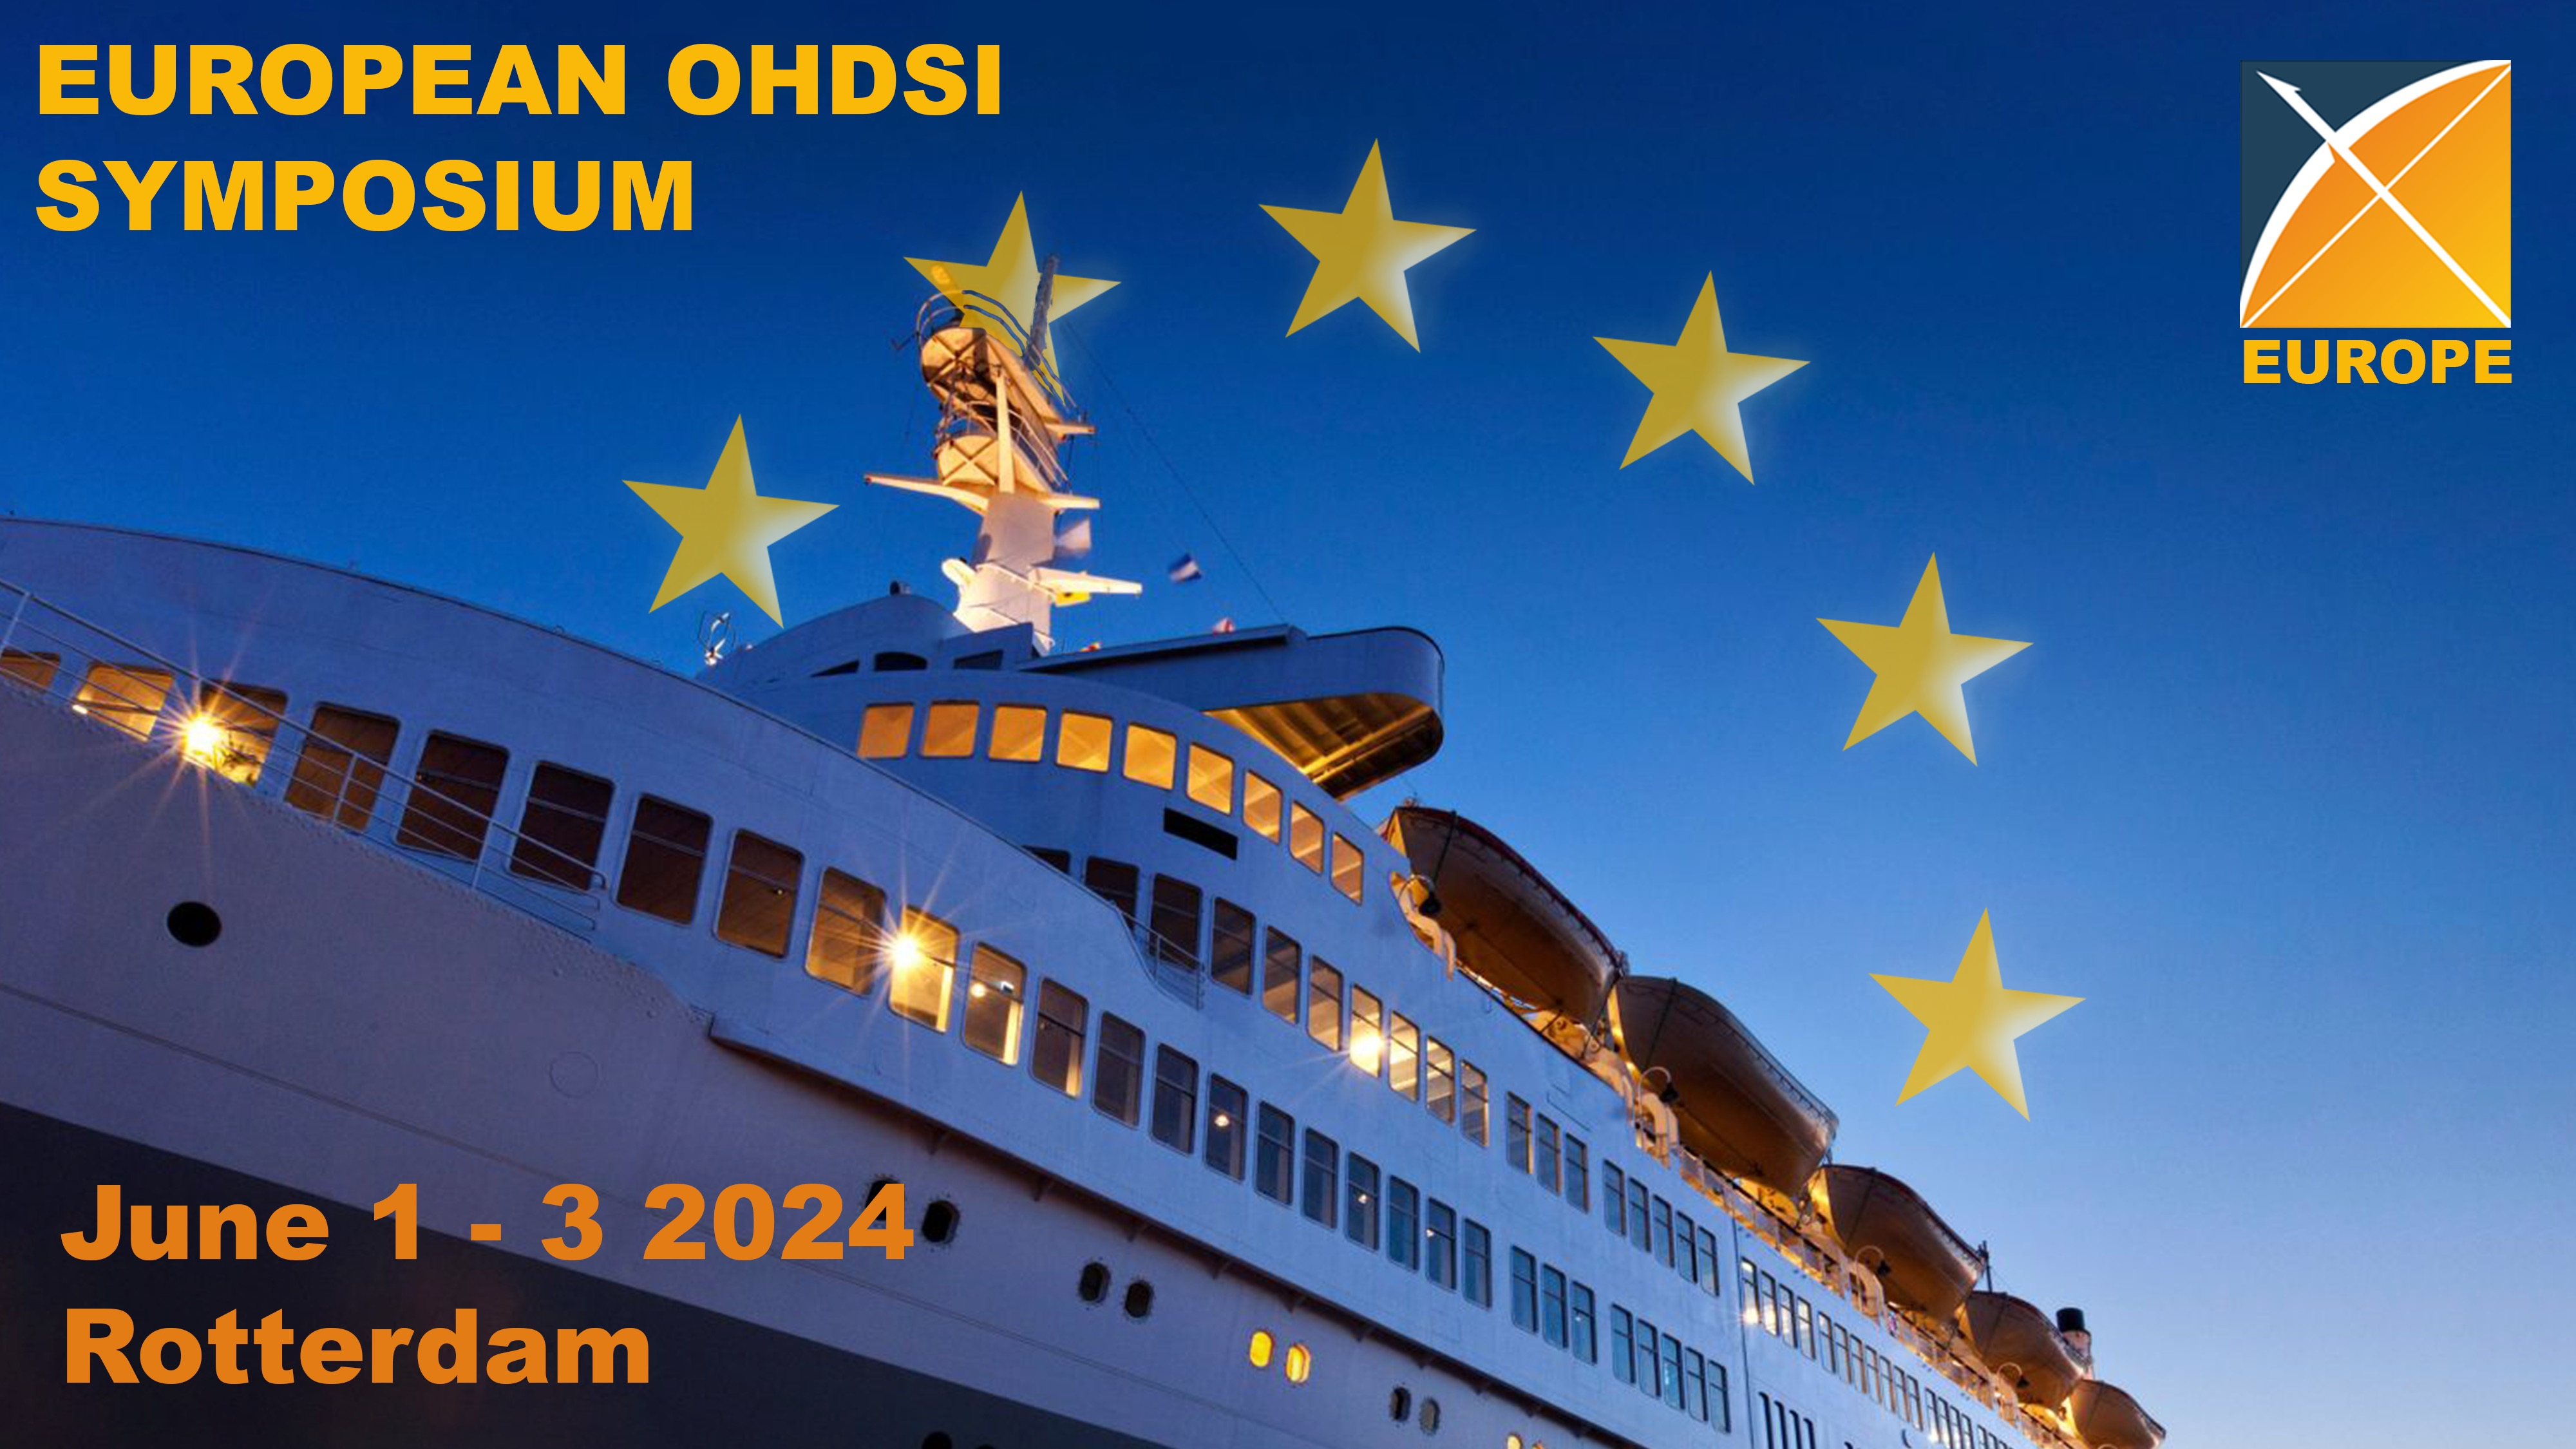
\includegraphics[width=0.70\textwidth]{figures/bannerSymposyum2024.jpg}
     \caption{Banner del Symposium Europeo 2024. Extraído de la web oficial \cite{OHDSIwebsite}}
    \label{fig:bannerSymposyum2024}
\end{figure}

Por ejemplo, en el Symposium Europeo del pasado año 2023, se presentaron proyectos relativos al almacenamiento de los datos de UCI en Holanda \cite{Jagesar2023The}, la integración del CDM de OMOP con el laboratorio de datos de salud alemám \cite{Finster2023Integrating}, la estandarización de la base de datos nacional francesa SNDS al modelo de OMOP \cite{Collumeau2023Standardization}, la armonización de los HCE hospitalarios en Ruanda al CDM \cite{Halvorsen2023Ruanda} y a la estandarización de los datos del registro europeo de sarcomas a OMOP \cite{vanSwieten2023Standardizing}, entre otros.

%La intención de esta sección es mostrar la gran relevancia que tiene actualmente la organización de OHDSI sobre todo en los grandes proyectos europeos. 

\section{¿Cómo generar evidencia?} \label{sec:05Evidencia}

Una vez que se conoce qué es OHDSI su misión y sus características fundamentales, se conoce la importancia de generar evidencia a partir del estudio de los datos clínicos. A continuación se exponen los principios fundamentales de la organización para generar evidencia confiable.

\subsubsection{The journey from data to evidence}

No es casualidad que la invitación que hace OHDSI a sus colaboradores lleve el slogan \textit{''Join the Journey''} sino que es un guiño al propósito al que se unen, es decir, al camino desde los datos hasta la evidencia o, en ingles, \textit{"The Journey from data to evidence"}.

\begin{figure}[H]
    \centering
    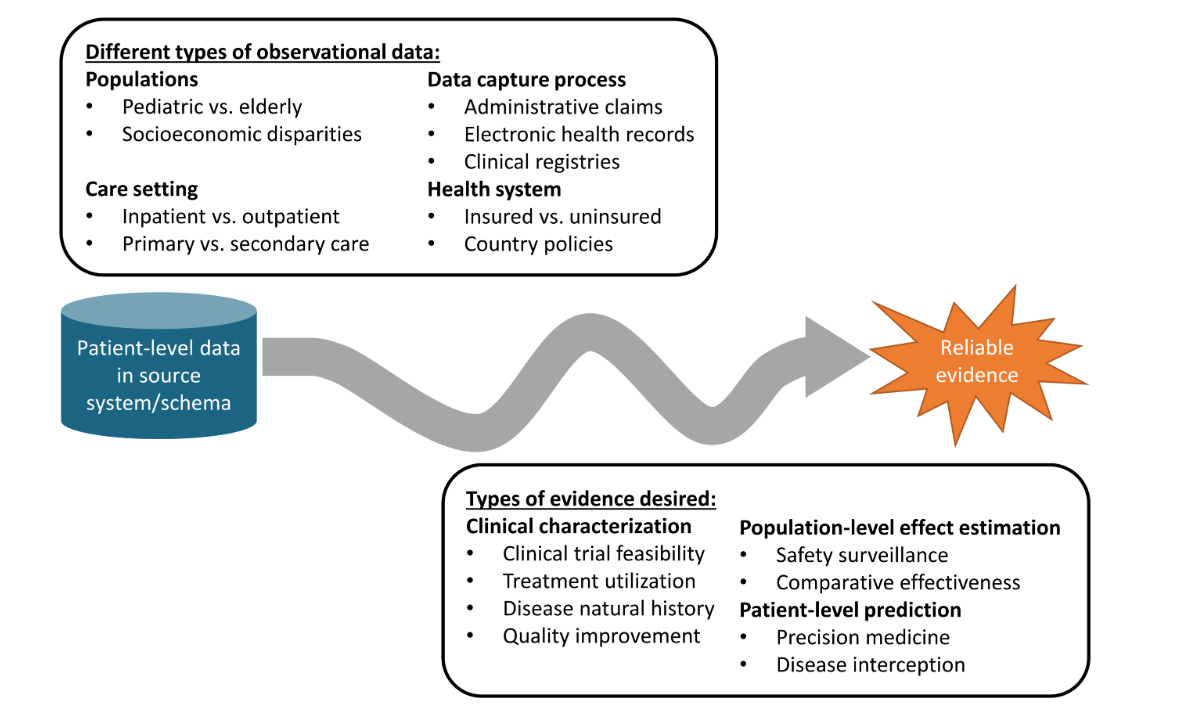
\includegraphics[width=0.80\textwidth]{figures/journeyDataToEvidence.png}
     \caption{\textit{The Journey from Data to Evidence}. Extraído del Libro de OHDSI \cite{OHDSIbook}}
    \label{fig:journeyDataToEvidence}
\end{figure}

La anterior Figura complementa a la Figura \ref{fig:drawinJourney} con mayor información sobre los diferentes tipos de datos que se almacenan y los diferentes tipos de evidencia que se quiere generar. Frente a la disparidad de los datos y la finalidad con la que son recodigos, OHDSI presentará el Modelo de Datos Común (véase \ref{subsec:05cdm}) y para la extracción de evidencia, la investigación metodológica mediante tres casos de uso fundamentales: la caracterización clínica de una cohorte, la estimación a nivel de población y la predicción a nivel de paciente (véase \ref{subsec:05investMetodolog}).

Los estudios que se llevan a cabo son estudios observacionales o fenotípicos, es decir, que simulan lo que sería un estudio clínico experimental sin intervención pero sobre datos ya almacenados de pacientes, en vez de realizar un seguimiento en vivo. De esta forma se logra obtener evidencia basada en datos. Cuando la evidencia se extrae sobre datos del mundo real (RWD), se denomina evidencia del mundo real (\textit{Real World Evidence, RWE}).

%De esta forma, OHDSI promueve una vía para generar evidencia interoperable entre las distintas organizaciones que interactúan a través de su red mundial, dicho de otra forma, pretende dar soporte para que miles de estudios diferentes sigan una misma metodología que facilite su comprensión de forma global.

Además, una característica fundamental de las investigaciones que se llevan acabo en OHDSI es que giran entorno al paciente, que es además el núcleo central del Modelo de Datos Común de OMOP. Por lo que un componente fundamental de cualquier investigación metodológica son las historias de los pacientes. \textbf{Para cada evento clínico que sucede se recoge una historia del paciente o \textit{Patient Journey}}. Es importante no confundir este concepto con la Historia Clínica Electrónica de un paciente (HCE) que recoge una ficha con todos los eventos que han le sucedido a lo largo de su vida. Las investigaciones observacionales se diseñan para extraer información sobre la recopilación de todos los \textit{patient journeys}.

\begin{figure}[H]
    \centering
    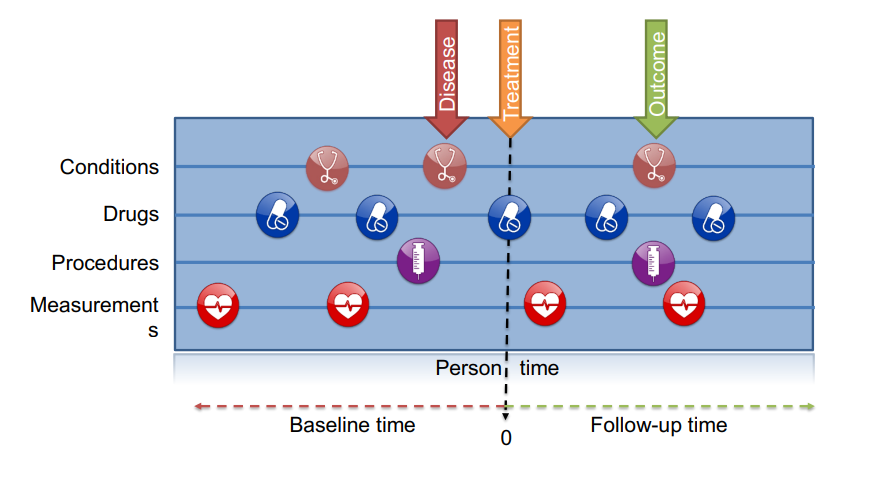
\includegraphics[width=0.80\textwidth]{figures/patientJourney.png}
     \caption{\textit{The patient Journey}. Extraído de la página web oficial \cite{OHDSIbook}}
    \label{fig:patientJourney}
\end{figure}

La historia del paciente,  como se muestra en la Figura \ref{fig:patientJourney}, es por tanto, una ventana temporal que recoge un evento clínico que le sucede a un paciente en un período de tiempo concreto. El evento se describe mediante tres períodos de tiempo: la enfermedad (rojo), el tratamiento (naranja) y el efecto (verde); y a partir de cuatro características esenciales: síntomas (\textit{conditions}), medicamentos (\textit{drugs}), procedimientos (\textit{procedures}) y pruebas (\textit{measurements}).

Los datos de pacientes se pueden agrupar en \textbf{cohortes} que comparten historias y características similares, al igual que a la hora de realizar un estudio clínico en vivo. Las diferentes  prácticas para los análisis de cohortes darán lugar a los diferentes tipos de evidencia deseada (caracterización, estimación a nivel de población, predicción a nivel de paciente). \textbf{Por tanto, el componente central para generar evidencia en OHDSI será la cohorte.}

%\begin{figure}[H]
%\centering
%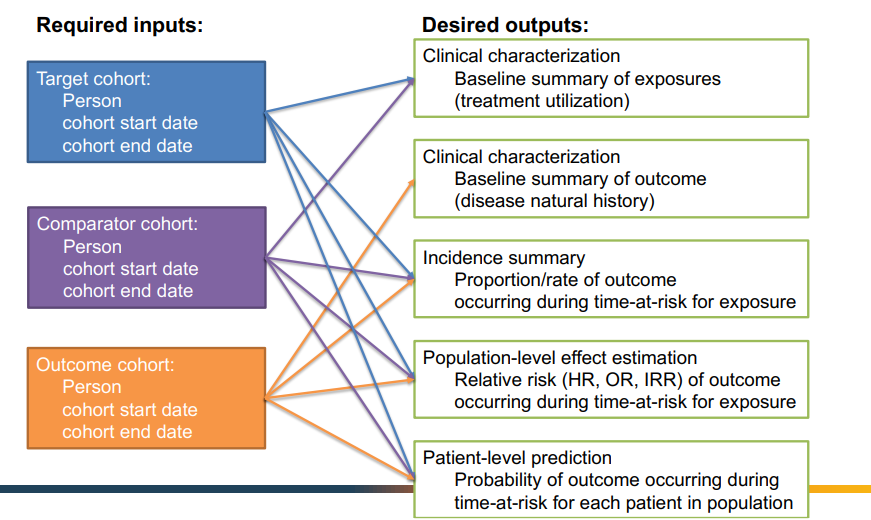
\includegraphics[width=0.70\textwidth]{figures/studyIO.png}
%     \caption{La definición de cohortes es el componente esencial para la generación de evidencia. Extraído del Tutorial2022 publicado en la web oficial \cite{OHDSIwebsite}}
%    \label{fig:studyIO}
%\end{figure}

\subsubsection{Implementación del análisis}

Para realizar un análisis, OHDSI distingue tres vías alternativas para generar la evidencia a partir de la base de datos estandarizada al OMOP CDM. Estas tres alternativas se muestran a continuación en la Figura \ref{fig:analysisImplementations}, extraída del capítulo 8 del Libro de OHDSI.

\begin{figure}[H]
    \centering
    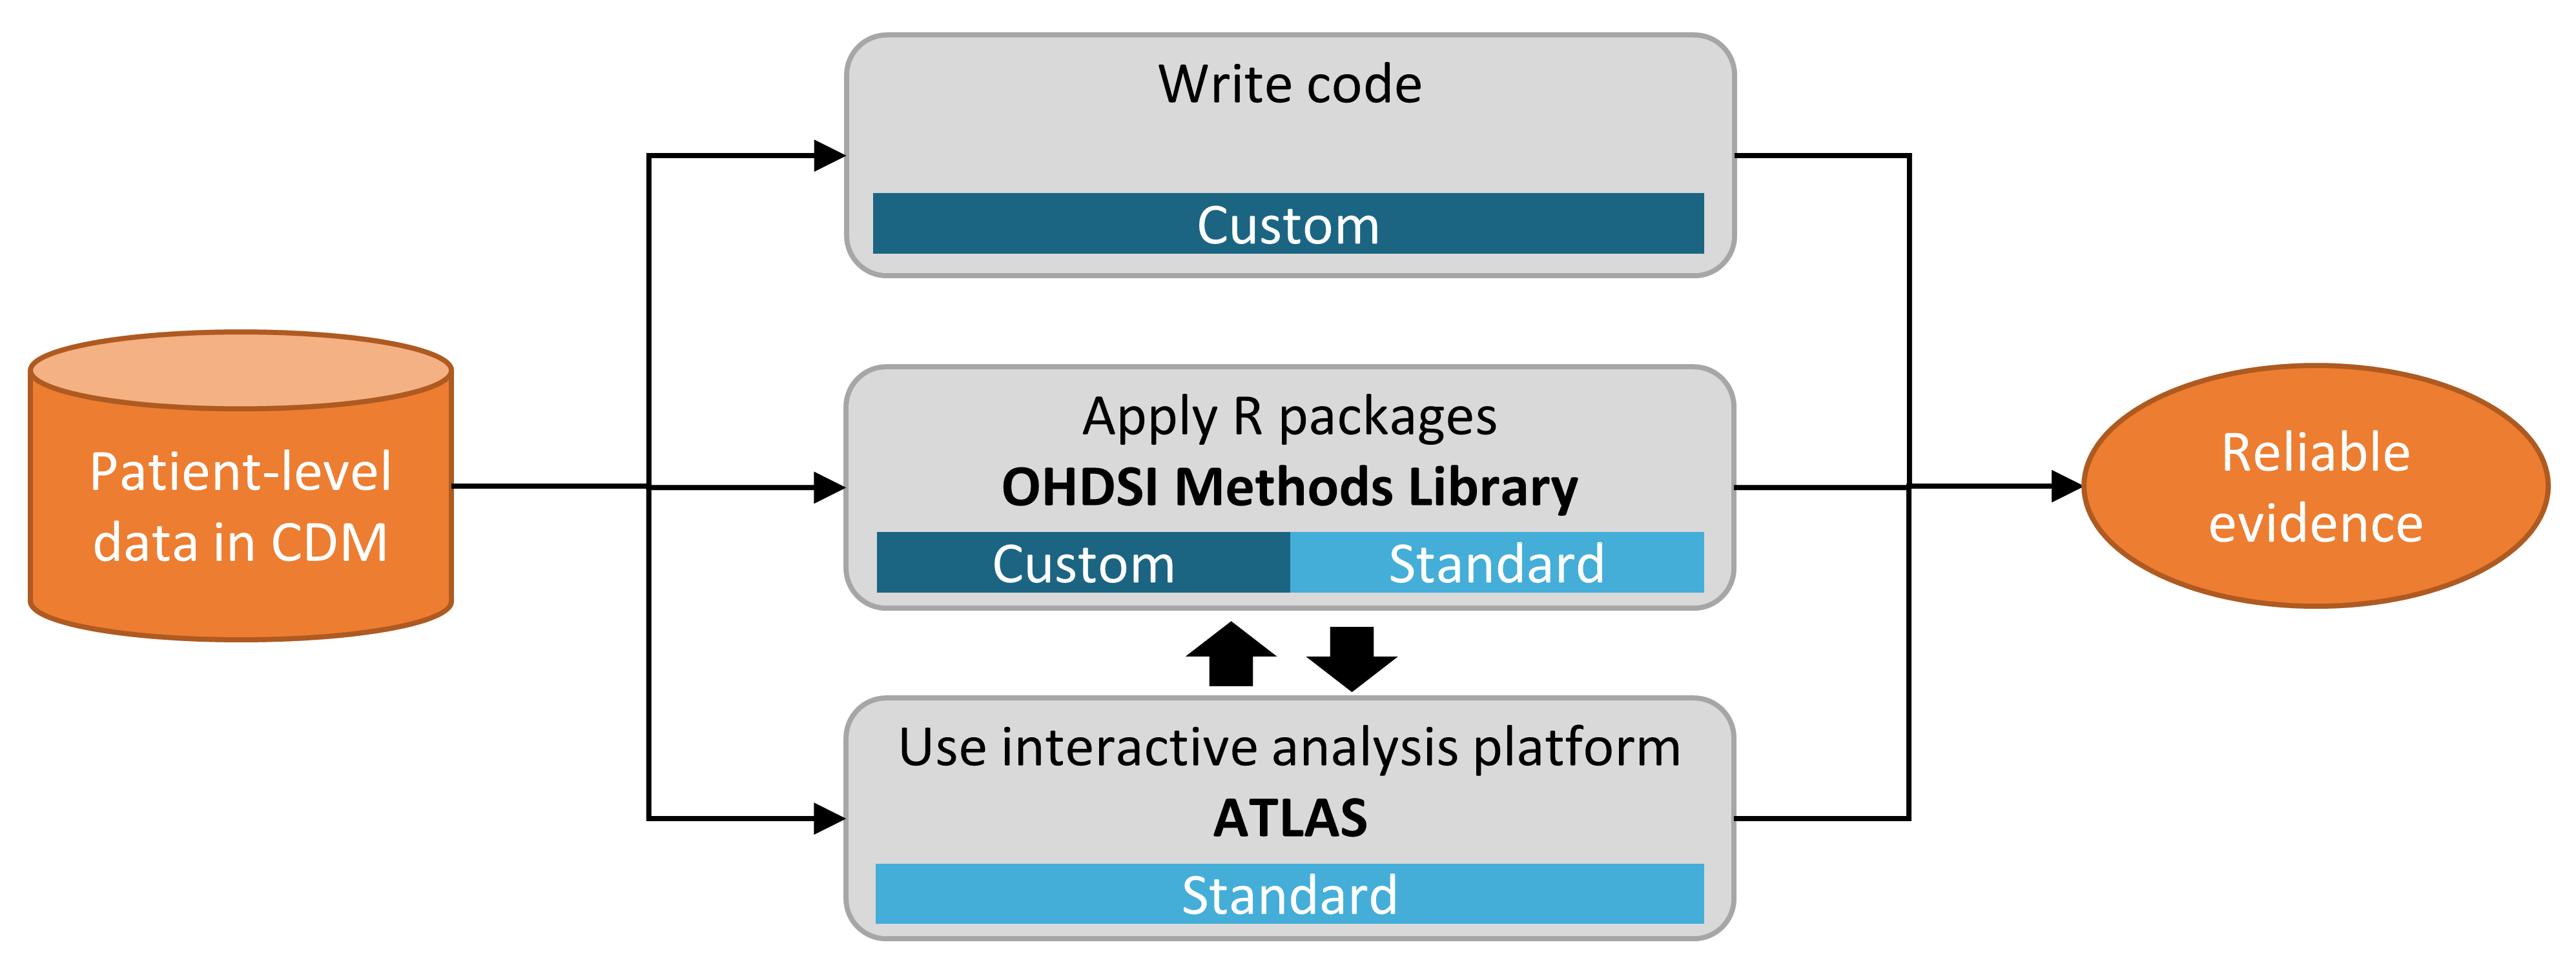
\includegraphics[width=0.80\textwidth]{figures/analysisImplementations.png}
     \caption{Tres vías para la implementación de un análisis observacional. Extraído del Libro de OHDSI \cite{OHDSIbook}}
    \label{fig:analysisImplementations}
\end{figure}

Cada vía se evalúa en cuanto a lo personalizada (\textit{custom}) o estandarizada (\textit{standard}) que es. A estas alturas se debe conocer que la vía más recomendada para implementar el análisis será la más estandarizada, es decir, la tercera vía.

La problemática que presentan la primera y la segunda vía consiste en ser en mayor o menor medida vías customizada, lo que genera problemas de interoperabilidad y reproducibilidad de los estudios. Si bien la primera vía consiste en la programación directa de código para realizar las consultas  (no hay ningún tipo de estandarización, distintos lenguajes de programación, funciones personalizadas) al menos la segunda vía hace uso de librerías estándares en R que OHDSI ofrece (\textit{OHDSI Methods Library}) pero, aunque se use el mismo lenguage de programación y funciones, los scripts pueden ser tan distintos que aún dificulten la interoperabilidad.

Por tanto, la tercera vía se presenta como la alternativa óptima por ser la más estandarizada y es la que empleará el TFG en el estudio práctico. Esto es, usar la herramienta interactiva \textit{low-code} de análisis de datos que ofrece OHDSI, denominada \textbf{ATLAS}, sin necesidad de programar directamente código.

%A partir de este momento se conoce que la implementación del estudio objeto del TFG se realizará a través de la herramienta de anális ATLAS, luego toda información a continuación está estrechamente ligada con su utilidad y uso en los análisis de ATLAS. Esta herramienta, junto a otras que también contribuyen a la estandarización del análisis se presentan en mayor detalle en \ref{sec:05herramientas}.

\section{Estándares}\label{sec:05estandares}

%\subsection{Estandarización de los datos} \label{subsec:05estandarDatos}

En términos de estandarización, OHDSI realiza una labor muy importante para paliar las dificultades de la investigación con datos de salud a causa de la heterogeneidad de los datos y estudios. Debido a la amplia colaboración internacional de la organización se recocone la necesidad de estándares que permitan el intercambio de información sin pérdida entre los distintos sistemas de información de los miembros.

La estandarización de la investigación en OHDSI se realiza en dos planos: a nivel de datos y a nivel de investigación. La estandarización a nivel de datos se realiza a través del uso del Modelo de Datos Común \ref{subsec:05cdm} y el Vocabulario \ref{subsec:05vocab} y la estandarización a nivel de investigación mediante la investigación metodológica \ref{subsec:05investMetodolog}.

\subsection{El Modelo de Datos Común} \label{subsec:05cdm}

El Modelo de Datos Común o \textit{Common Data Model (CDM)} de OMOP es ''un estándar de datos comunitario abierto, diseñado para estandarizar la estructura y el contenido de los datos de observación y permitir análisis eficientes que puedan producir evidencia confiable'' \cite{gitPagesCMD}, en definitiva, es un modelo semántico estándar para estructurar los datos de salud. La información más relevante y actualizada sobre el CDM se encuentra en su página de github \cite{gitPagesCMD} y en el capitulo 4 del Libro de OHDSI \cite{OHDSIbook}.

\subsubsection{Características}

El modelo de datos de OMOP presenta características importantísimas para hacer frente a las necesidades del panorama socio-sanitario actual presentado en \ref{sec:01Contexto}. A continuación se presentan las características más relevantes del modelo (extraídas de la sección  4.1 del Libro de OHDSI \cite{OHDSIbook}), según las necesidades identificadas previamente.

\begin{itemize}
    \item \textbf{Estructura diseñada para la investigación}. 
    El modelo presenta una estructura única y óptima para un propósito concreto: el de facilitar la realización de estudios observacionales. Por tanto reduce notoriamente los desafíos relativos a las diferentes estructuras y propósitos con los que se recogen los datos clínicos.
    \item \textbf{Modelo centrado en el paciente}. Es un modelo centrado en el paciente (alineado con la msima característica de la Sanidad 4.0). Estructuralmente esto significa que todos los eventos y tablas están relacionados con la tabla central del paciente, denominada \textit{Person}. 
    \item \textbf{Protección y privacidad}. El modelo limita el acceso a la información personal de los pacientes, evitando en la medida de lo posible el acceso a información personal sensible como nombres o fechas de nacimiento, para fomentar la protección y privacidad de los datos. Mayor información sobre las técnicas empleadas para ello se encuentran en el apartado \textit{Privacidad del paciente y OMOP} de la página de github \cite{gitPagesCMD}.
    \item \textbf{Reutilización de estándares}. Un aspecto importantísimo es que el modelo propone su propio estándar pero sin olvidar los estándares globalmente utilizados, de manera que integra y reutiliza los conceptos provenientes de estándares ya existentes (ej. SNOMED, LOINC...) referenciándolos en su propio Modelo de Datos Común. El conjunto de todos los estádnares existentes adheridos al modelo de OMOP conforma el Vocabulario.
    \item \textbf{Neutralidad tecnológica}. El modelo no requiere una tecnología específica sino que puede estructurarse en cualquier base de datos relacional (ej. Oracle, SQL Server...), ajustándose a los requisitos tecnológicos necesarios de cada organización (identificado también como una dificultad en \ref{sec:01Contexto}).
    
\end{itemize}

\subsubsection{Modelo de Datos Lógico}

Actualmente el CDM ha lanzado ya su sexta versión, sin embargo, esta aún no está soportada por todas las herramientas de la comunidad, por lo que se sigue sugiriendo el uso del CDM v5.4, que es la última versión completamente funcional. 

A la hora de realizar un estudio en ATLAS o cualquier otra herramienta del ecosistema OHDSI la base de datos estará necesariamente estandarizada a este modelo por lo que es importante conocer su estructura fundamental. A continuación, en la Figura \ref{fig:cdm54} se presenta la estructura lógica de este modelo y en la Figura \ref{fig:cdm_ER} como modelo Entidad-Relación. Adicionalmente existe una página web que proporciona un modelo interactivo para facilitar su estudio \cite{CDMinteractive}.

Aunque el modelo de datos común de OMOP es muy complejo, incluso existen grupos de trabajo de la comunidad (\textit{workshops}) especializados sólo en este ámbito, en esta subsección tan solo se van a presentar los conceptos más estrictamente necesarios para la comprensión subyacente del contenido del TFG.

\begin{figure}[H]
    \centering
    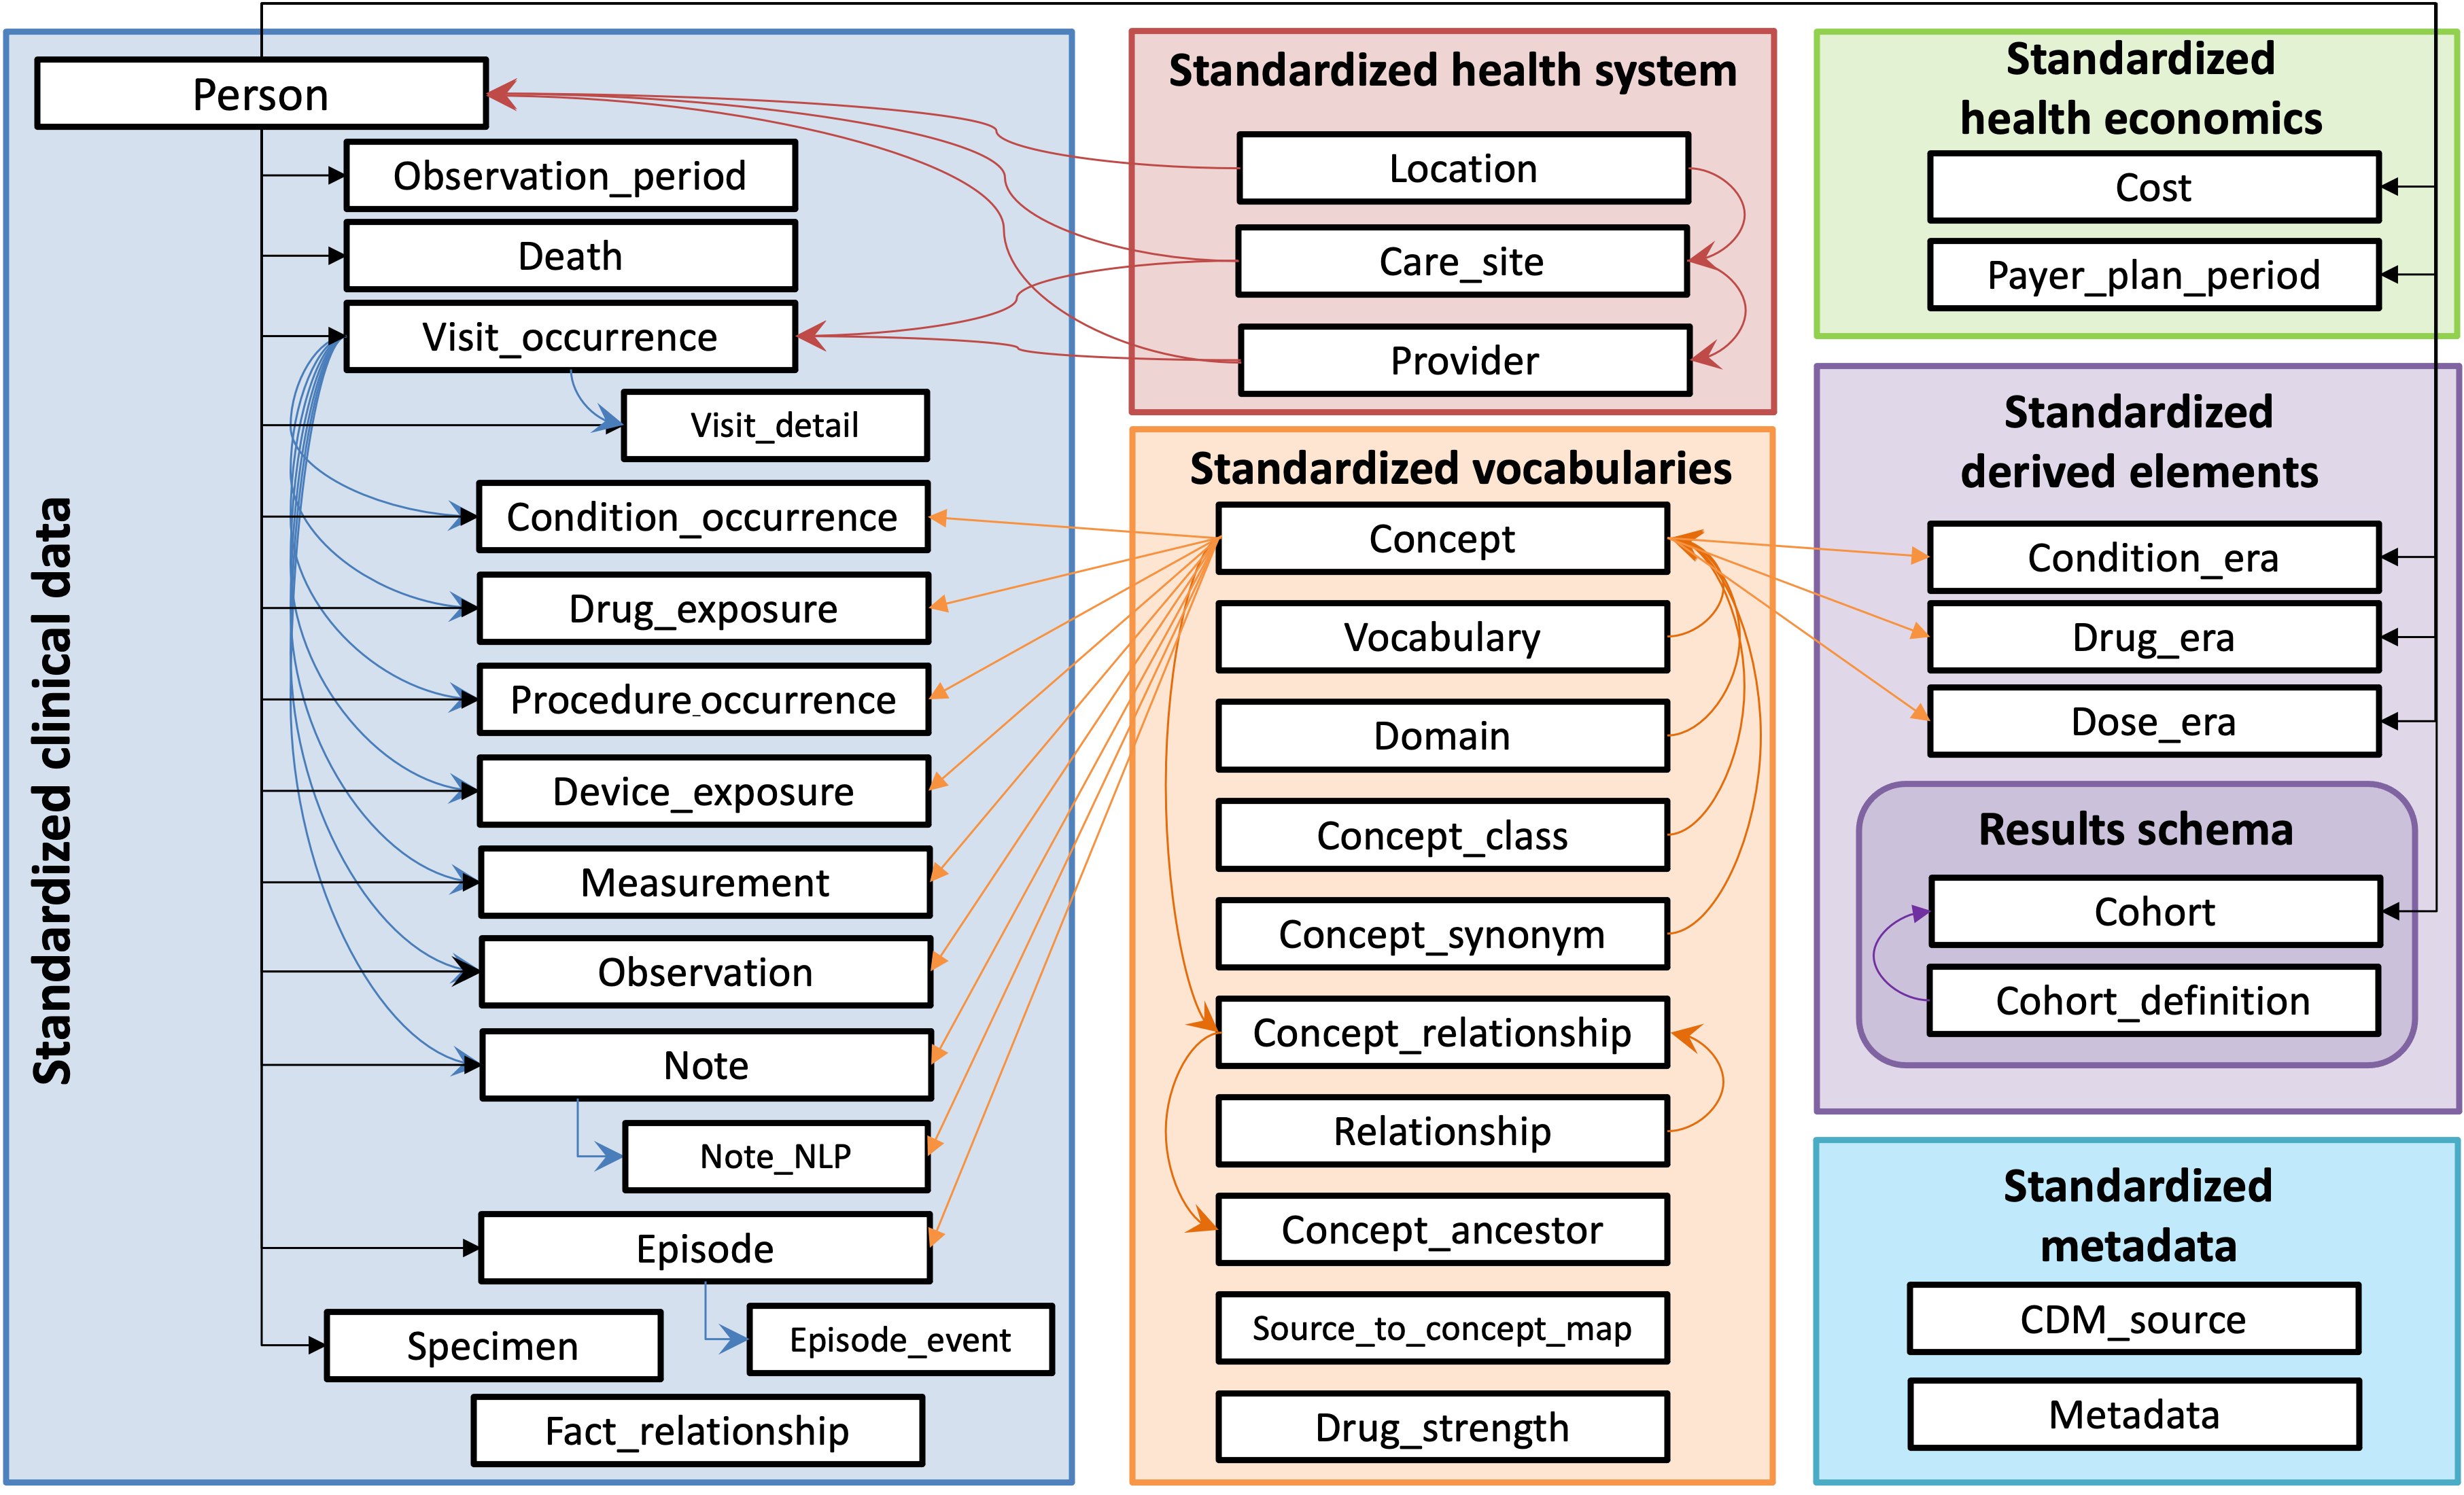
\includegraphics[width=0.90\textwidth]{figures/cdm54.png}
     \caption{Estructura del CDM v5.4. Extraída de la página de github del CDM \cite{gitPagesCMD}}
    \label{fig:cdm54}
\end{figure}

\begin{figure}[H]
    \centering
    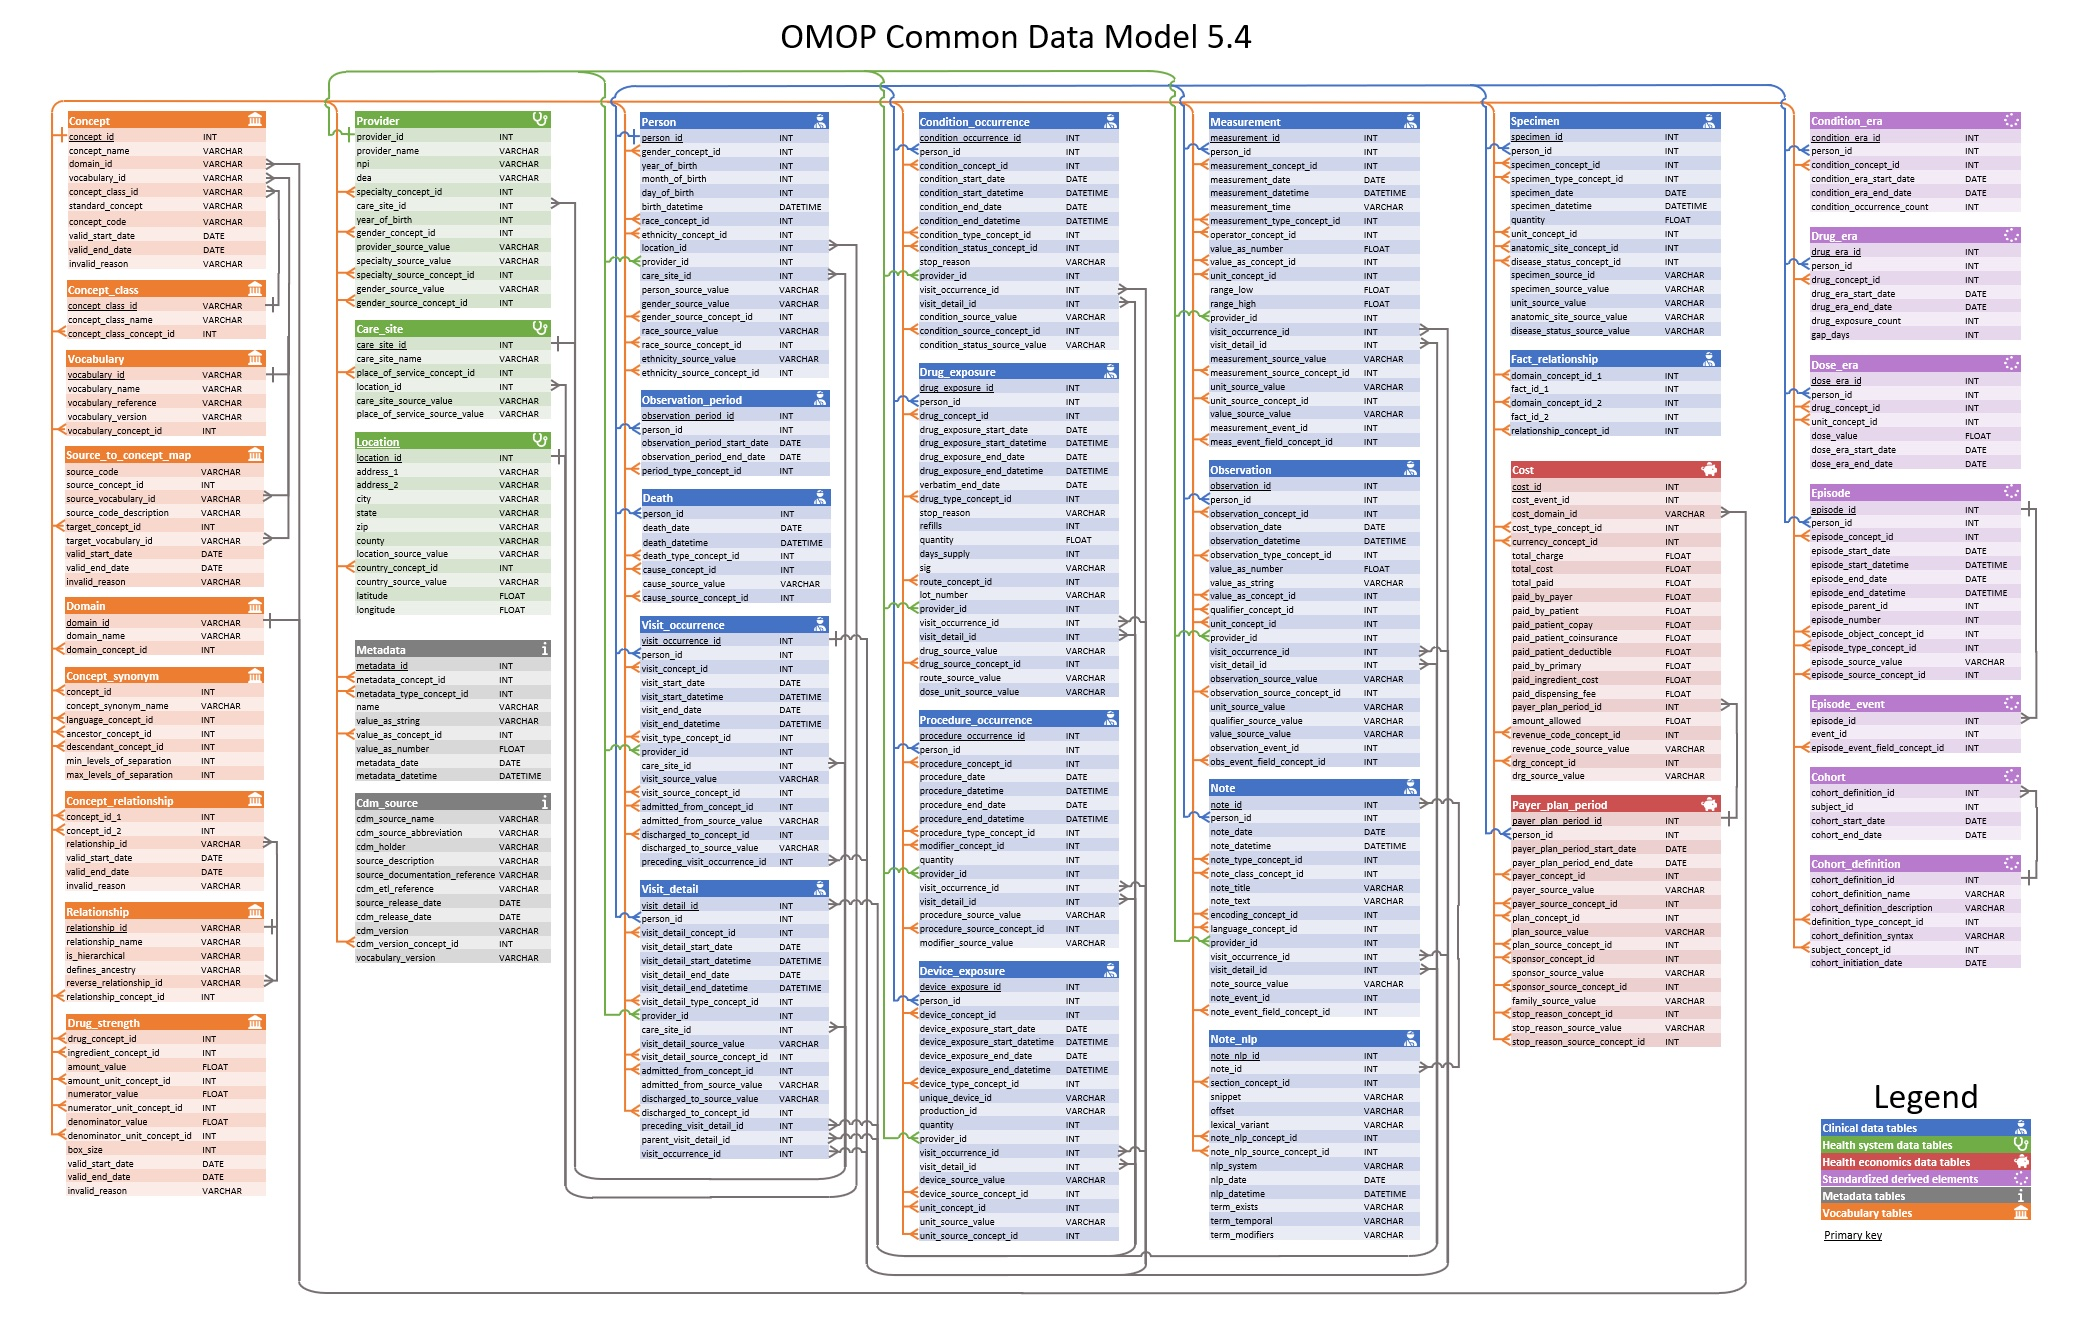
\includegraphics[width=1\textwidth]{figures/cdm_ER.jpg}
     \caption{Modelo Entidad-Relación del CDM v5.4. Extraída de la página de github del CDM \cite{gitPagesCMD}}
    \label{fig:cdm_ER}
\end{figure}

El modelo se comprende de 39 tablas agrupadas en seis grupos, de los cuales se destaca la importancia de tres: Datos clínicos estandarizados (\textit{Standardized clinical data}, en azul), Vocabularios estandarizado (\textit{Standardized vocabularies}, en naranja), Elementos derivados estandarizados (\textit{Standardized derived elements}, en morado). El grupo más importante es el de datos clínicos, que contiene la tabla Persona (\textit{Person}), su relevancia se debe a la característica centrada en el paciente del modelo.

Cada evento clínico se registra en el modelo como un \textbf{Concepto} (\textit{Concept}), perteneciente al grupo del vocabulario estandarizado. Además, cada concepto está ligado a un \textbf{Dominio} que especifica a qué tipo de información clínica corresponde dicho concepto. A continuación se muestra una tabla con los 30 dominios existentes y la cantidad de conceptos que tiene asociado cada uno.

\begin{figure}[H]
    \centering
    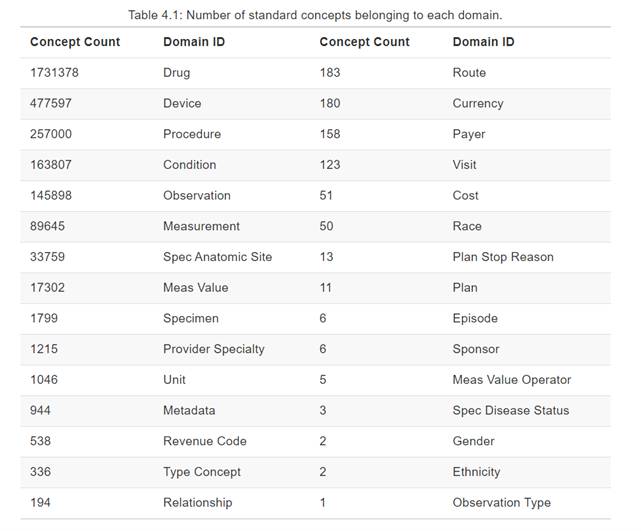
\includegraphics[width=0.80\textwidth]{figures/cdm_domains.png}
     \captionof{table}{Dominios del CDM v5.4. Extraída del Libro de OHDSI \cite{OHDSIbook}}
    \label{fig:cdm_domains}
\end{figure}

La información que contiene cada dominio se puede inferir fácilmente de la traducción al español del nombre por lo que no se va a hacer hincapié en ello. No obstante, se puede encontrar más información en \cite{OHDSIbook}, \cite{gitPagesCMD} o \cite{CDMinteractive}.

\subsection{El Vocabulario}\label{subsec:05vocab}

El Vocabulario es otro de los elementos centrales del Modelo de Datos Común de OMOP y una gran herramienta de estandarización e interoperabilidad entre sistemas. Como se ha comentado en varias ocasiones, actualmente hay muchos estándares distintos en funcionamiento que establecen las terminologías de los eventos clínicos (por ejemplo LOINC, SNOMED CT, RxNorm...). El beneficio del Vocabulario de OMOP es que integra todos los vocabularios ya existentes en un único \textbf{Vocabulario estándar}, a través de la referenciación entre \textbf{conceptos estándar} (pertenecientes a OMOP) y conceptos no estándar (pertenecientes a vocabularios alternativos).

El Vocabulario de OHDSI, por tanto, impera sobre un conjunto de vocabularios, respetando las diversas procedencias de cada término pero mapeándolos a un único vocabulario estándar. \textbf{Cada concepto no estándar está asociado a un concepto estándar} y esta es la clave del Vocabulario. 

Como todas las herramientas de la comunidad, la información acerca de este está disponible online de forma pública en el capítulo 5 del Libro de OHDSI \cite{OHDSIbook} y en la página de github del CDM \cite{gitPagesCMD}. Por otra parte, existe un buscador online de términos en el Vocabulario de OMOP denominado ATHENA \cite{ATHENAweb}. 

\begin{figure}[H]
\centering
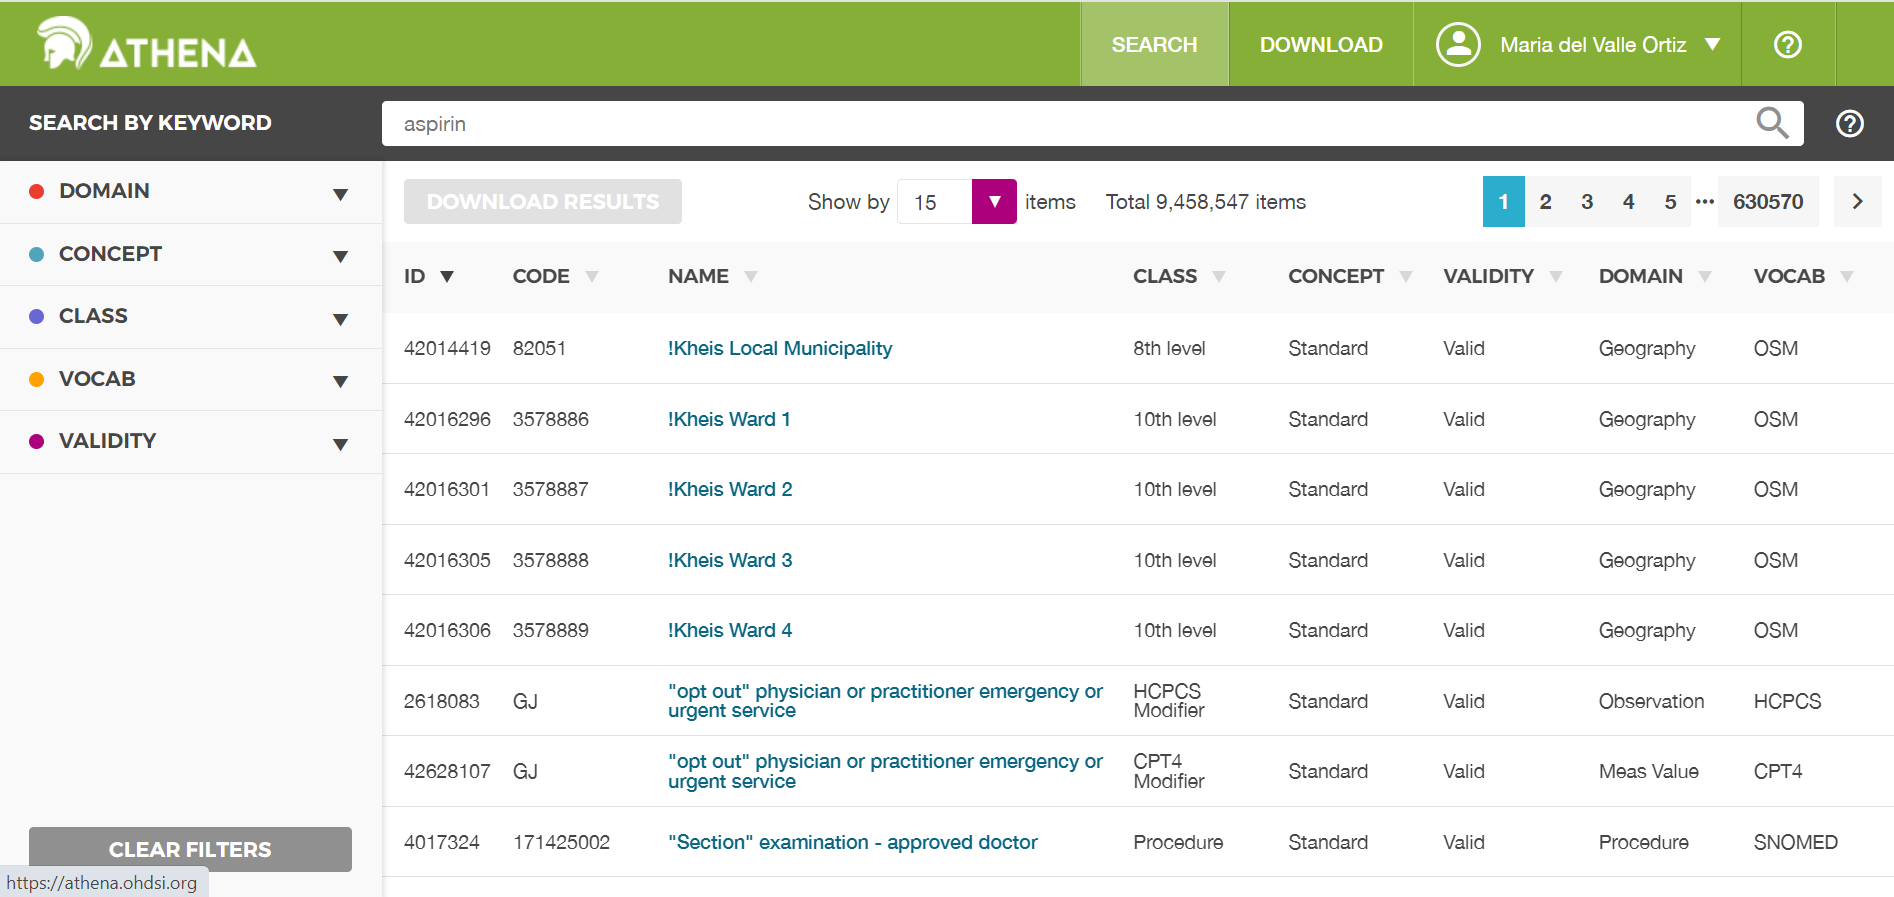
\includegraphics[width=0.90\textwidth]{figures/ATHENAcap.png}
     \caption{Captura de pantalla del menú principal de ATHENA}
    \label{fig:ATHENAcap}
\end{figure}

Actualmente hay más de nueve millones de términos registrados en el Vocabulario de OMOP, como se muestra en la Figura \ref{fig:ATHENAcap}, y 155 vocabularios distintos coexisten juntos en el estándar, de los cuales al menos 30 son vocabularios internos de OMOP.

%\textcolor{red}{- lA RELACIÓN QUE GUARDAN LOS CONCEPTOS ENTRE SÍ ES JERARQUICA}


\subsection{Investigación metodológica} \label{subsec:05investMetodolog}

Con el fin de estandarizar y proveer un marco metodológico en el camino hacia la generación de evidencia, OHDSI define tres casos de usos que establecen los fines investigacionales sobre los datos del \textit{Common Data Model}: (i) la caracterización, (ii) la estimación a nivel de población (iii) la predicción a nivel de paciente. 

\begin{figure}[H]
\centering
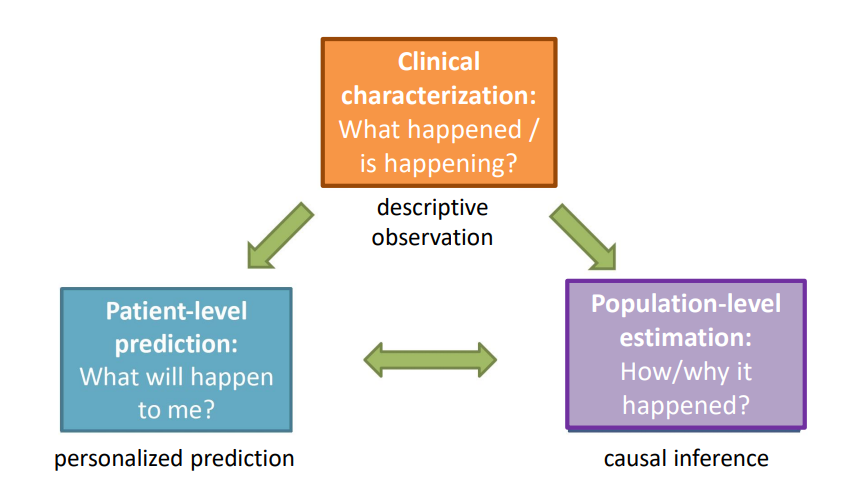
\includegraphics[width=0.80\textwidth]{figures/useCases.png}
     \caption{Esquema simplificado de los casos de uso para la investigación en OHDSI. Extraído del Symposium 2023, publicado en la web oficial \cite{OHDSIwebsite}}
    \label{fig:useCases}
\end{figure}

Estos tres casos de uso se presentan generalmente en los \textit{Symposium} y \textit{Workshops}, para dar a conocer a la comunidad el esquema propio de investigación de OHDSI. Además el Libro de OHDSI \cite{OHDSIbook} los presenta de forma general en el capítulo 7 y de forma específica para cada caso de uso en los capítulos 11, 12 y 13, respectivamente. A continuación se muestra otro esquema más complejo también presentado en el Symposium 2023 en el que se encuadra cada caso de uso en la ventana temporal que encuadra un estudio observacional.


\begin{figure}[H]
\centering
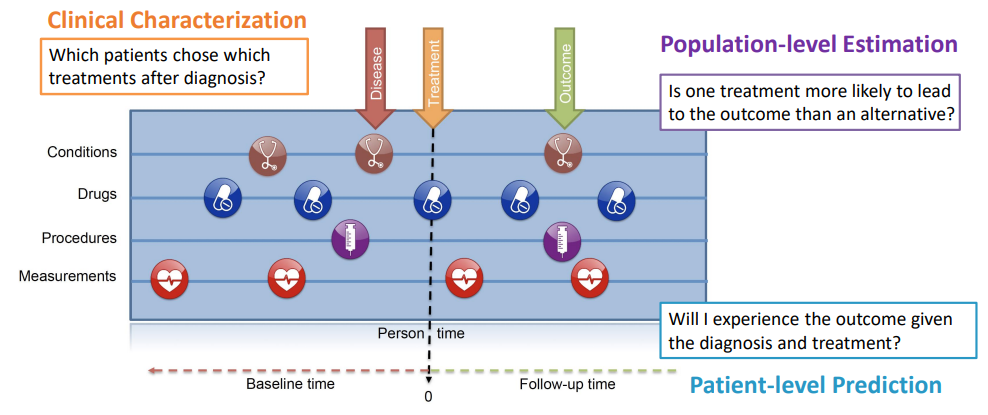
\includegraphics[width=0.70\textwidth]{figures/useCasesJourney.png}
     \caption{Esquema de los casos de uso encuadrado en la historia del paciente. Extraído del Symposium 2023 publicado en la web oficial \cite{OHDSIwebsite}}
    \label{fig:useCasesJourney}
\end{figure}

\subsubsection{Cohortes}

\textcolor{red}{Añadir explicación más detallada con conceptos relevantes cuando empiece a manejar ATLAS}

\begin{figure}[H]
\centering
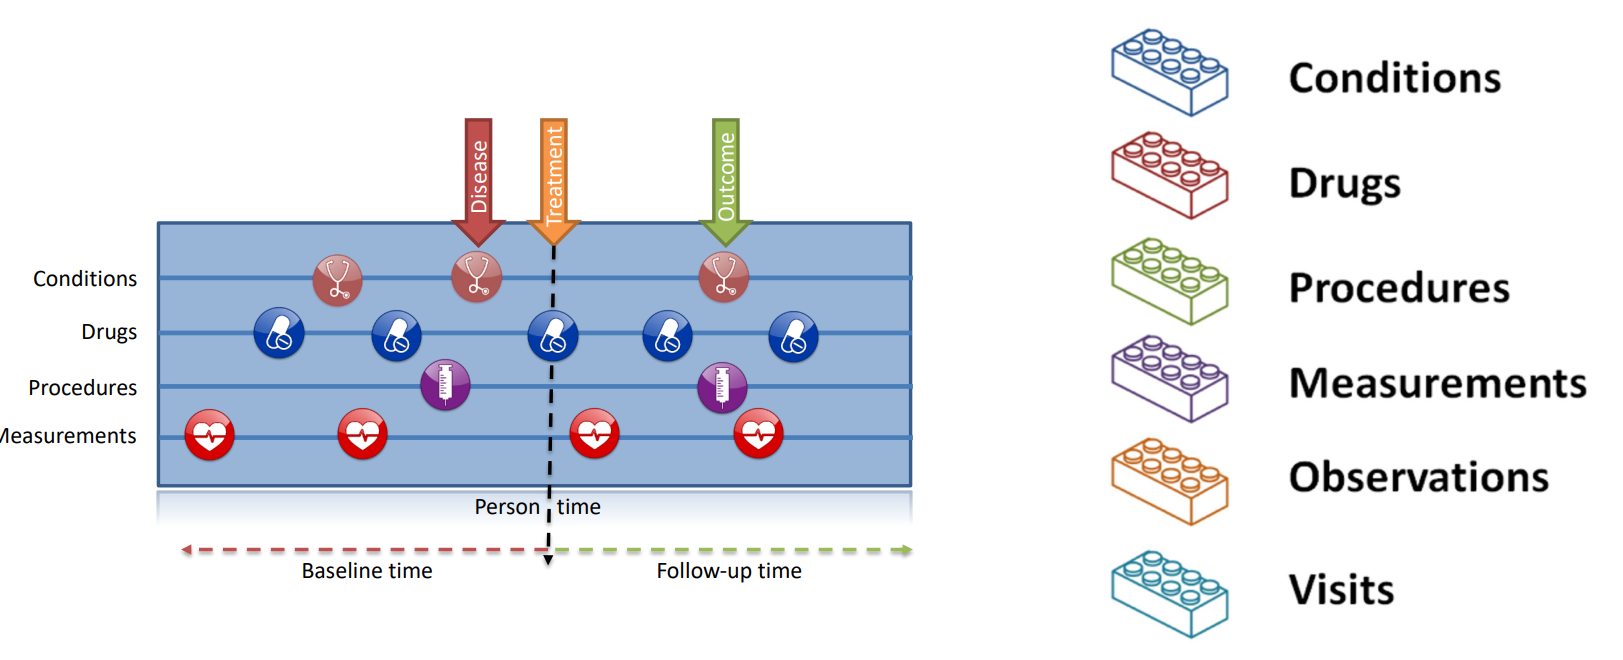
\includegraphics[width=0.70\textwidth]{figures/bblocksPatientJourney.png}
     \caption{Building blocks para la definición de una cohorte. Extraído del Tutorial 2022 publicado en la web oficial \cite{OHDSIwebsite}}
    \label{fig:bblocksPatientJourney}
\end{figure}


\subsubsection{Caracterización}

\textcolor{red}{Añadir explicación más detallada con conceptos relevantes cuando empiece a manejar ATLAS}

La caracterización busca la caracterización a nivel estadístico de un cohorte o una base de datos. Es una mera descripción estadística de los datos, sin realizar inferencias, predicciones o análisis más complejos, simplemente observando la base de datos.

La caracterización consiste en caracterizar una población a través de métricas estadísticas descriptivas con el objetivo de formular hipótesis sobre los determinantes de la salud y la enfermedad.

\subsubsection{Estimación a nivel de población}

\textcolor{red}{Añadir explicación más detallada con conceptos relevantes cuando empiece a manejar ATLAS}

La estimación a nivel de población busca realizar inferencias causales sobre los efectos de las intervenciones sanitarias en la población. Se pretende entender los efectos causales para comprender las consecuencias de las acciones

\subsubsection{Predicción a nivel de paciente}

\textcolor{red}{Añadir explicación más detallada con conceptos relevantes cuando empiece a manejar ATLAS}

La predicción a nivel de paciente busca, en base a los datos obtenidos de los conjuntos de pacientes en la base de datos, realizar predicciones concretas para un individuo concreto.

\section{Herramientas} \label{sec:05herramientas}

OHDSI proporciona un conjunto de herramientas para facilitar la realización de los estudios e investigaciones a raíz de los datos clínicos y fomentar la interoperabilidad entre estos, aportando un estándar de herramientas. 

Las herramientas que proporciona la organización están disponibles públicamente online y de forma gratuita y son desarrolladas por los propios miembros de la comunidad. Entre todas las herramientas, para la realización de este Trabajo Fin de Grado se destaca la herramienta de análisis de datos clínicos ATLAS \ref{subsec:05ATLAS}, aunque también existen otras herramientas importantes de forma indirecta \ref{subsec:05otrasHerramientas}.

\subsection{ATLAS} \label{subsec:05ATLAS}

ATLAS es la herramienta de OHDSI por excelencia porque es la que estandariza el análisis observacional una vez que la base de datos está convertida al modelo OMOP. La documentación oficial sobre ATLAS se encuentra en el capítulo 8 del Libro de OHDSI y en su repositorio de github \cite{githubATLAS}. Además, aparte de la documentación oficial, hay montones de información esparcidas por la red sobre ATLAS, en publicaciones científicas, foros de OHDSI, videotutoriales en youtube y un largo etcétera.

\begin{figure}[H]
\centering

\includegraphics[width=0.25\textwidth]{figures/ATLASlogo.png}
     \caption{Logo de ATLAS. Extraída del repositorio de github \cite{githubATLAS}}
    \label{fig:ATLASlogo}
\end{figure}

Un importante promotor del uso de ATLAS es la red europea de datos EHDEN \cite{ehden} (véase \ref{sec:01EstadoArte}). En esta línea, también la plataforma EHDEN Academy también ofrece cursos gratuitos sobre el uso de ATLAS y otras herramientas OHDSI.

\subsubsection{Características y beneficios de su uso}

El uso de ATLAS es beneficioso para la comunidad científica debido principalmente a su naturaleza \textit{open-source}, \textit{low-code} y la reproducibilidad que ofrece para los estudios:

\begin{enumerate}[label=\roman*.]

    \item \textbf{Open source}. ATLAS se presenta como una herramienta disponible públicamente online, configurable gracias a su característica de cógido abierto, que expone toda su información y el propio código que la compone en los repositorios de github de la organización y, por si fuera poco, cuenta con el apoyo de un equipo de desarrolladores pendiente en los foros e \textit{issues} que se reportan vía github para solucionar las dudas que tengan los implementadores. 

    \item \textbf{Low-code}. Por otro lado, no requiere de conocimientos expertos de programación, puesto que es \textit{low-code}. La herramienta se implementa sobre la Biblioteca de Métodos de OHDSI, con soporte para análisis en R, pero no requiere programación directa sino que ofrece una interfaz gráfica e intuitiva para el analista de datos. Además, el código que subyace al análisis es fácilmente exportable, siempre estructurado según el mismo estándar, favoreciendo la interoperabilidad del mismo.

\begin{figure}[H]
\centering
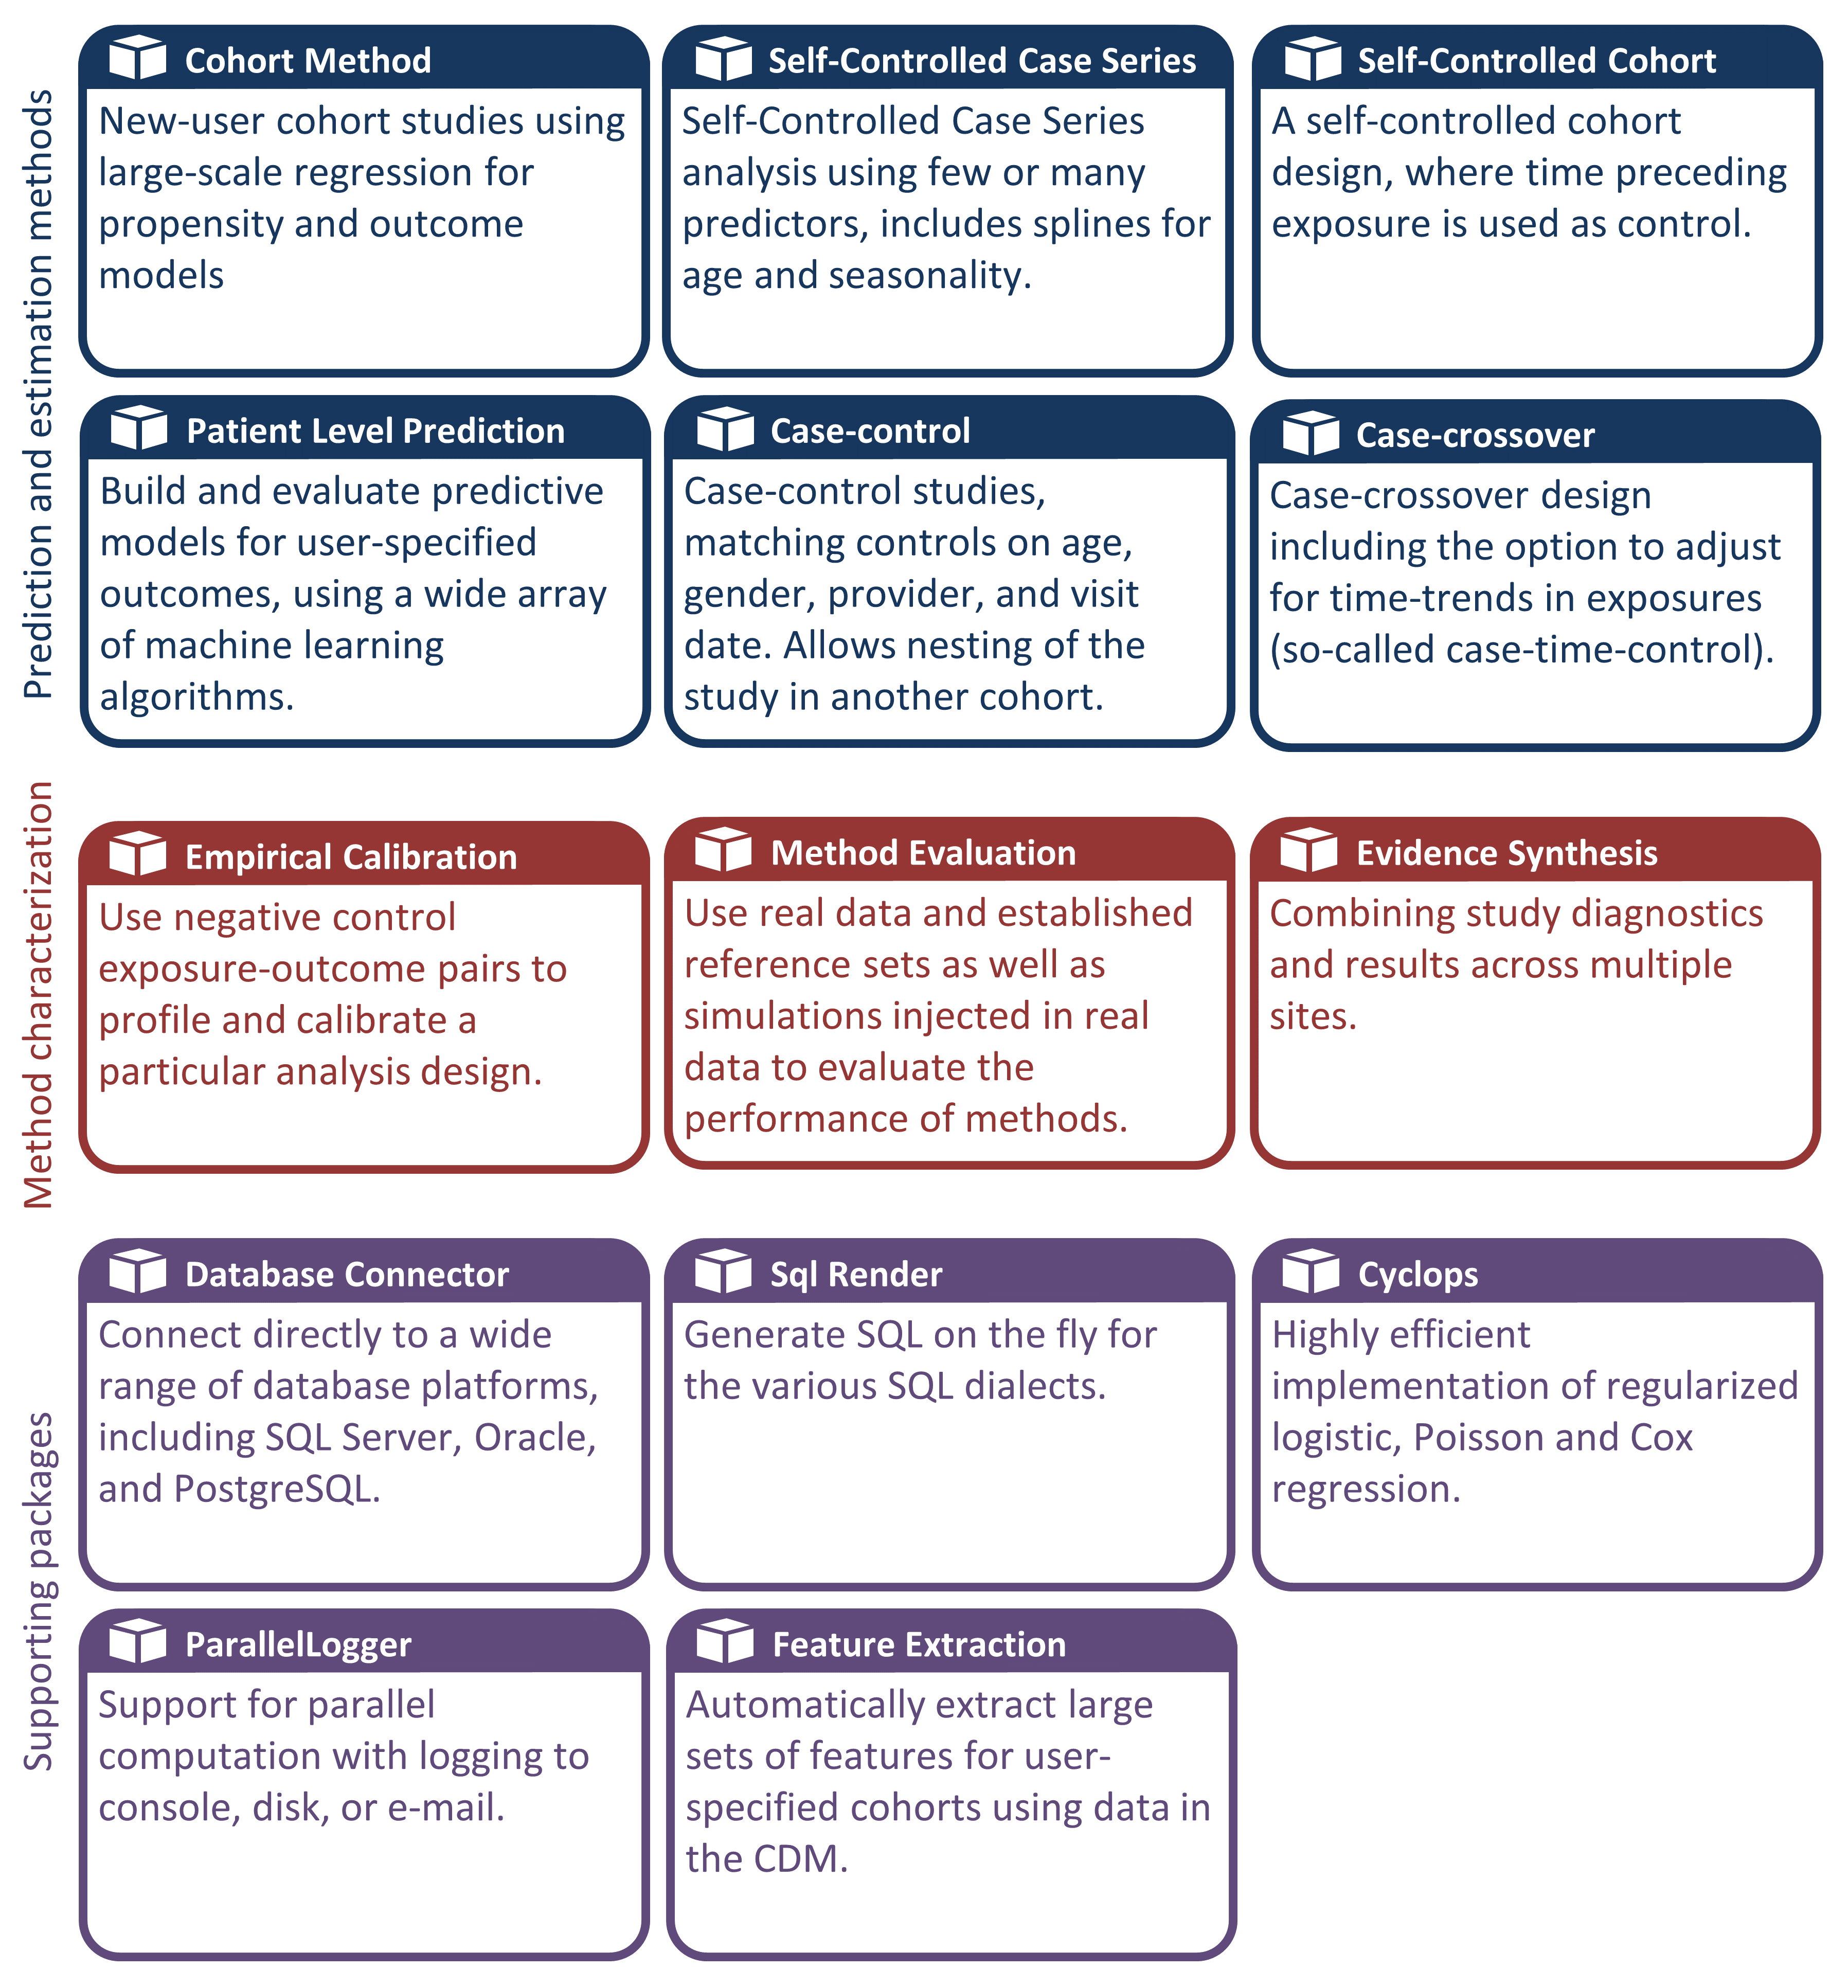
\includegraphics[width=0.50\textwidth]{figures/methodsLibrary.png}
\caption{Biblioteca de Métodos OHDSI que utiliza ATLAS. Extraída del Libro de OHDSI \cite{OHDSIbook}}
\label{fig:methodsLibrary}
\end{figure}
    
     Todo ello no solo facilita la tarea del analista de datos sino que además favorece la interoperabilidad entre los estudios, puesto que todos los estudios que utilizan ATLAS implementan (en una capa inferior) los mismos métodos, el mismo lenguaje de programación y la misma estructura de análisis (véase \ref{sec:05Evidencia}). 

     \item \textbf{Reciclabilidad}. Por último, otro beneficio es que gracias a estas características ATLAS permite diseñar estructuras para el estudio de los datos que puedan utilizarse en diferentes bases de datos distintas. Volviendo al ejemplo de la plancha en \ref{sec:05Evidencia}, esto quiere decir que una misma plancha (o estudio) puede conectarse a cualquier enchufe de cualquier región (a cualquier base de datos). ATLAS está intrínsicamente configurada para diseñar análisis reproducibles, por lo que los elementos que se configuran durante un análisis de datos (grupos de cohortes, estimadores, predictores, grupos de conceptos...) se pueden exportar fácilmente a modo de estructura general e implementarse sobre otro estudio que, aunque posea datos distintos ejecute ATLAS. Por tanto las estructuras más eficientes que se utilizen en un análisis remoto, pueden compartirse en la red de la comunidad y ser utilizados en cualquier nodo y cualquier estudio, favoreciendo la reciclabilidad, reproducibilidad e interoperabilidad del estudio.
    
\end{enumerate}

\subsubsection{Aspectos técnicos}

En cuanto a los aspectos técnicos, ATLAS se despliega como una herramienta basada en web, normalmente alojada en un servidor Apache, combinada con la WebAPI de OHDSI. Generalmente se recomienda su despliegue en Google Chrome. Además la herramienta puede implementarse de forma pública a través de internet o tras el firewall de la red privada de una organización, según las necesidades de la entidad que lo implementa.

Sin embargo, es importante recalcar que tanto ATLAS como la mayoría de las herramientas de OHDSI no consiste en un archivo ejecutable aislado sino en una aplicación contenida y dependiente de un ecosistema completo basado en web. La dependencia principal y red que sostiene a ATLAS es la \textbf{WebAPI}.

\begin{figure}[H]
    \centering
    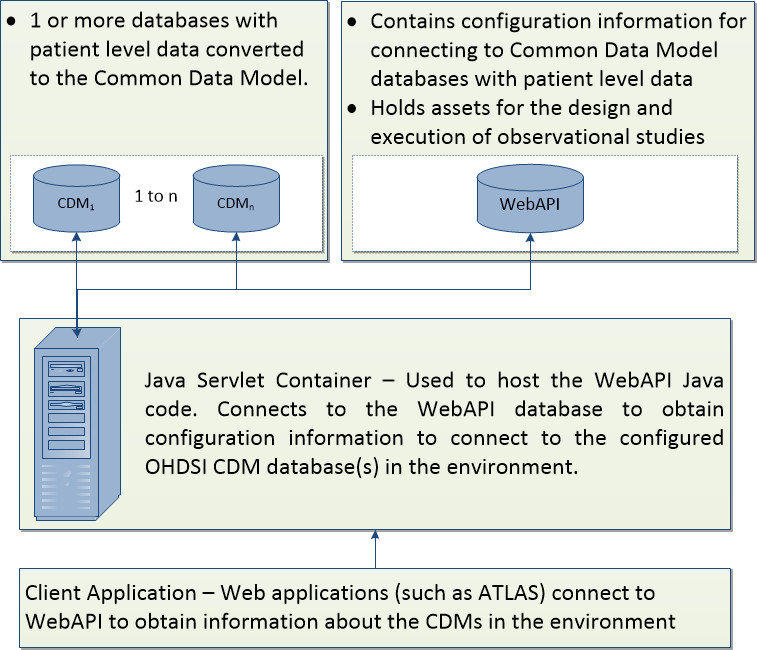
\includegraphics[width=0.50\textwidth]{figures/webAPIwiki.png}
     \caption{Estructura de la WebAPI. Extraída de la wiki de github \cite{githubWebAPIwiki}}.
    \label{fig:webAPIwiki}
\end{figure}

Tal y como se muestra en la Figura \ref{fig:webAPIwiki}, la Web API es la aplicación que proporciona los servicios RESTful para que la herramienta pueda interactuar con las bases de datos \cite{githubWebAPIwiki}. Por tanto su relación con ATLAS es estrictamente necesaria. ATLAS no es una herramienta aislada sino un eslabón del ecosistema OHDSI.

Por otra parte, la herramienta en sí se muestra a través de una interfaz gráfica, que proporciona un estrecho menú lateral con 15 herramientas para el análisis de datos. La interfaz de la herramienta seleccionada se muestra en el lado derecho, como se muestra en la Figura \ref{fig:ATLASdemoHome}.

\begin{figure}[H]
\centering
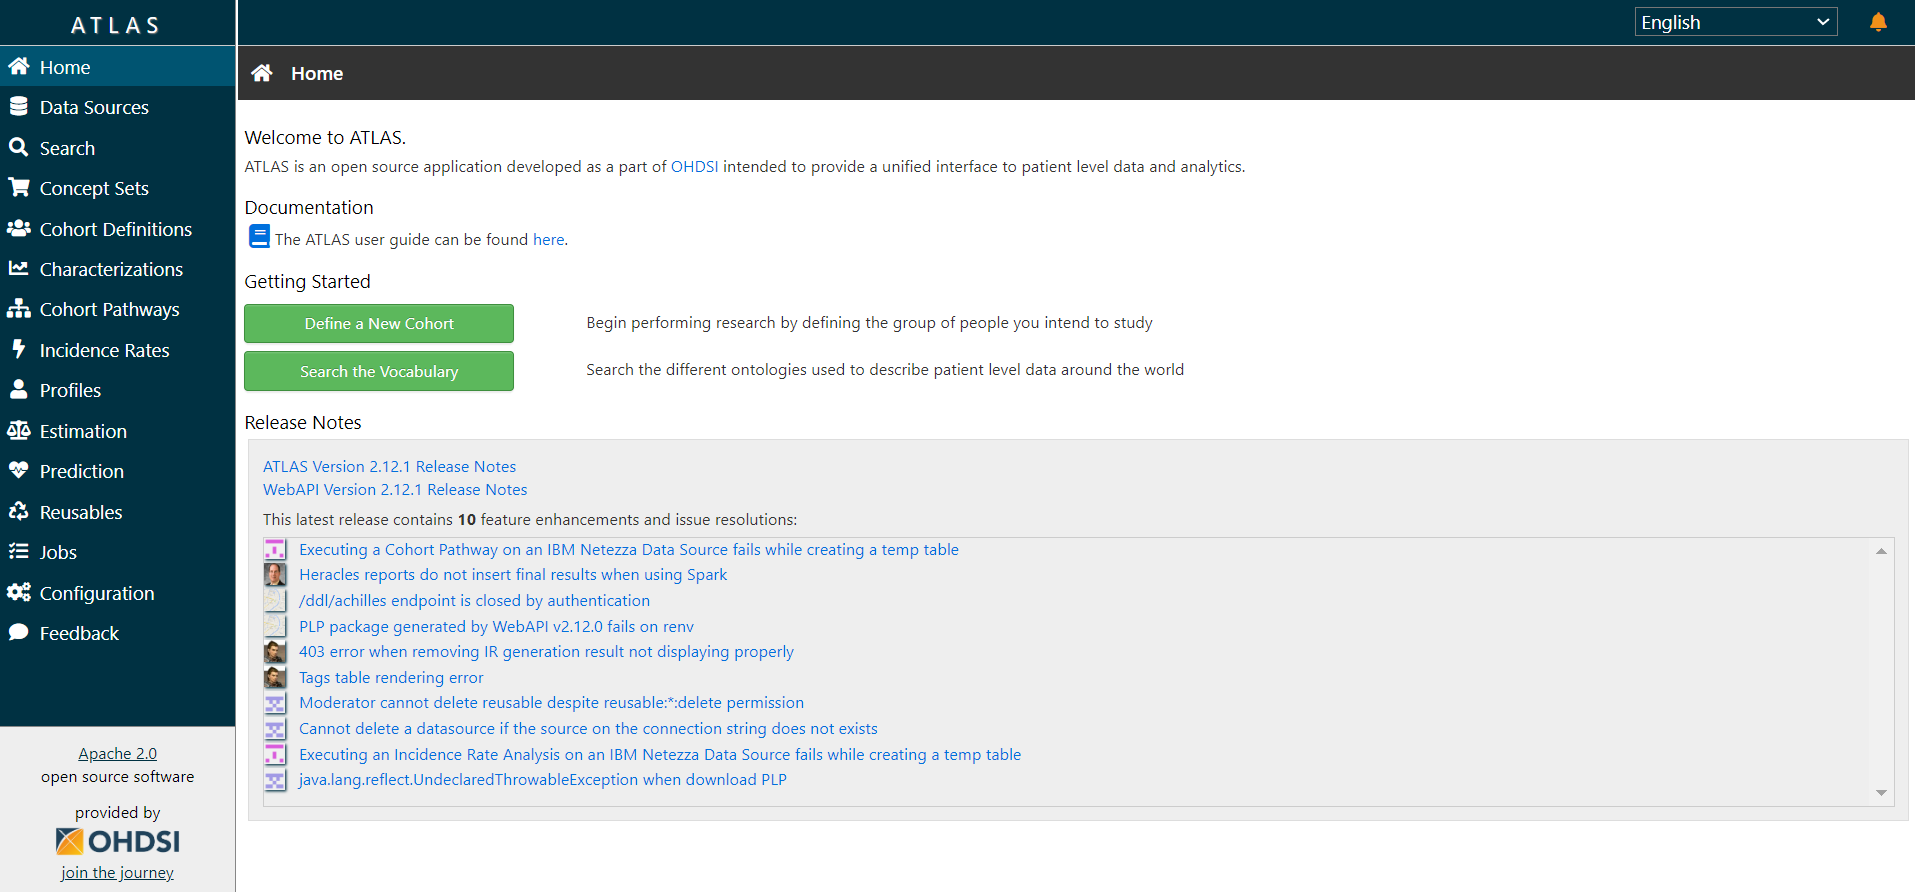
\includegraphics[width=0.90\textwidth]{figures/ATLASdemoHome.png}
     \caption{Captura de pantalla del menú principal de ATLAS demo}
    \label{fig:ATLASdemoHome}
\end{figure}

Recientemente, en diciembre de 2023, ATLAS lanzó su versión 2.14.1 que está en correcto funcionamiento y es la que se utiliza en el desarrollo del Trabajo Fin de Grado. Más información sobre los aspectos técnicos de la herramienta se encuentran en el repositorio de github \cite{githubATLAS}.

\subsubsection{Estrategias de Implementación}

La implementación de ATLAS en una organización puede ser una tarea complicada por su dependencia con la WebAPI, la Biblioteca de Métodos y otras dependencias al ecosistema OHDSI. 

No obstante, la organización ha desarrollado varias iniciativas que facilitan su implementación y accesibilidad, para no crear obstáculos en la promoción del uso de la herramienta. Estas iniciativas se describen a continuación.

\begin{enumerate}[label=\alph*.]

    \item \textbf{ATLAS demo} \cite{ATLASdemo}. En primer lugar, esta es una herramienta muy fácilmente accesible que proporciona la comunidad científica para tomar un primer contacto con la herramienta. En este caso, la herramienta es accesible a través del navegador web, publicamente a través de Internet. Cualquier usuario de internet tiene acceso a la herramienta demo. Se le denomina demo porque se sobreentiende que su uso es principalmente educativo o formativo, aunque verdaderamente ofrece todas las capacidades de la herramienta y los análisis que con ella se realizan, podrían reutilizarse en estudios más complejos o de organizaciones privadas.

    \item \textbf{ATLAS Docker}. Por otro lado, también muy fácilmente implementable se presenta \textbf{Broadsea} \cite{githubBroadsea}, que consiste en la virtualización del ecosistema OHDSI en un multicontenedor Docker. Gracias a la facilidad del uso de las tecnologías Docker, esta forma de implementar el ecosistema es bastante sencilla, permitiendo además añadir nuevas configuraciones más complejas (si fuese necesario) añadiendo o eliminando contenedores. Para realizar la parte práctica de este trabajo se emplea la tecnología Docker de Broadsea para implementar ATLAS. A la herramienta ATLAS desplegada con Broadsea, frecuentemente se le denominará a lo largo del documento \textit{ATLAS Broadsea}. El TFG presenta un documento anexo bastante complejo enteramente dedicado a la instalación, despliegue y configuración del entorno Broadsea (véase anexo \ref{anexo:manual}). Además, la arquitectura de Broadsea también se presenta en \ref{cap:07diseño}.

    \item \textbf{ATLAS Amazon Web Services}. Otra alternativa que propone la organziación, en colaboración con Amazon, es la virtualización del ecosistema en el entorno de computación en la nube de Amazon Web Services (AWS). Para ello se ofrecen los entornos \textit{OHDSI-in-a-Box} \cite{githubOHDSIBox} y \textit{OHDSIonAWS} \cite{githubOHDSIAWS}. OHDSI-in-a-Box se crea específicamente como un entorno de aprendizaje y se utiliza en la mayoría de los tutoriales proporcionados por la comunidad OHDSI mientras que OHDSIonAWS es una arquitectura de referencia para entornos OHDSI de clase empresarial, multiusuario, escalables. Por las restricciones intrínsecas al uso de AWS, estas alternativas han sido rechazadas para ser empleadas en el TFG.
    
    \item \textbf{ATLAS Azure}. Por último, \textit{OHDSI on AZURE} \cite{OHDSIonAzure} es otra alternativa de virtualización pero a través de la plataforma Microsoft de Azure. No obstante, esta alternativa es la menos común.
    
\end{enumerate}

\subsubsection{Herramientas embebidas}

Si bien las herramientas del ecosistema de OHDSI no son totalmente aisladas, ATLAS presenta en su propia interfaz acceso a dos de estas herramientas de forma íntegra, para facilitar la eficiencia y rapidez en el análisis. Estas herramientas son las siguientes:

\begin{itemize}

    \item \textbf{ACHILLES} \cite{githubACHILLES}. Esta herramienta, de las siglas \textit{Automated Characterization of Health Information at Large-Scale Longitudinal Evidence Systems}, en español Caracterización automatizada de la información sanitaria en sistemas de evidencia longitudinal a gran escala, sirve para caracterizar y/o obtener un reporte estadístico de la base de datos estandarizada que se va a utilizar para el estudio. Intrínsicamente es una librería de R que se implementa como una opción del menú lateral \textit{Data Sources} de ATLAS.
    \item \textbf{ATHENA} \cite{githubATHENA}. Esta herramienta sirve para realizar búsquedas dinámicas en el Vocabulario de OMOP (véase \ref{subsec:05vocab}). Está implementada en ATLAS en la opción \textit{Search} del menú lateral. Además, se puede acceder a ella online de forma externa a través de su propia página web \cite{ATHENAweb}.
    
\end{itemize}


\subsection{Otras herramientas} \label{subsec:05otrasHerramientas}

El ecosistema de OHDSI presenta gran cantidad de herramientas adicionales. A continuación se presentan otras herramientas que aunque no se utilizan directamente, son importantes para realizar un análisis de datos completo. 

\begin{itemize}
    
    \item \textbf{HADES} \cite{githubHADES}. HADES, del inglés\textit{ Health Analytics Data-To-Evidence Suite} y en español Suite de análisis sanitario de datos a evidencia, es el nombre con el que se denomina a la herramienta que implementa el paquete R con la Biblioteca de Métodos de OHDSI (ver Figura \ref{fig:methodsLibrary}). Se puede instalar como un entorno independiente mediante Java y Rtools para implementar análisis mediante código estandarizado (véase Figura \ref{fig:analysisImplementations}). No se utiliza en el TFG más alla de la implementación subyacente de las bibliotecas en ATLAS.
    \item \textbf{Rabbit tools y Usagi} \cite{OHDSIsoftTools}. Estas herramientas en conjunto llevan a cabo el proceso de ETL, para omopizar las bases de datos al Modelo de Datos Común de OMOP. Las herramientas son tres: White-Rabbit, Rabbit-In-Hat y Usagi. No se utiliza directamente en el TFG porque el dataset utilizado para el análisis ya estaba previamente omopizado.
    \item \textbf{Data Quality Dashboard} \cite{githubDQD}. Esta herramienta, en español Panel de control de calidad de los datos, pertenece a un paquete de HADES aunque implementado como una interfaz gráfica aparte para facilitar su acceso online. Tal y como su nombre indica sirve para automatizar la tarea de comprobación de la calidad de los datos, un paso previo fundamental antes de realizar un análisis de datos. Tampoco se utiliza directamente para el TFG porque este estudio se llevó a cabo durante la omopización del dataset.
        
\end{itemize}

\section{Conclusiones} \label{sec:05conclusion}

En este capítulo se concluye la relevancia de OHDSI en el panorama sanitario y tecnológico actual, capaz de subsanar las necesidades del mismo a través de su misión, estándares y herramientas (\ref{sec:05OHDSI}, \ref{sec:05estandares}, \ref{sec:05herramientas}).

Principalmente se realiza una labor importantísima de estandarización, tanto a nivel de datos mediante el Modelo de Datos Común \ref{subsec:05cdm} y el Vocabulario \ref{subsec:05vocab} como a nivel de estudios \ref{subsec:05investMetodolog} mediante la Investigación metodológica y sobre todo gracias al auge del uso de su herramienta estrella, ATLAS \ref{subsec:05ATLAS}, que se emplea para el estudio práctico del TFG.